%%%%%%%% ICML 2019 EXAMPLE LATEX SUBMISSION FILE %%%%%%%%%%%%%%%%%

\documentclass{article}

% Recommended, but optional, packages for figures and better typesetting:
\usepackage{microtype}
\usepackage{booktabs} % for professional tables


\usepackage{graphicx} % "demo" option just for this example
\usepackage{subcaption}

\usepackage{amsmath}
\usepackage{booktabs,subcaption,amsfonts,dcolumn}
\newcolumntype{d}[1]{D..{#1}}
\newcommand\mc[1]{\multicolumn{1}{c}{#1}} % handy shortcut macro

\graphicspath{{/home/danai/Documents/ANN_latex/images/Report1Exercise2/}{/home/danai/Documents/ANN_latex/images/Report3}}

\usepackage{hyperref}

% Attempt to make hyperref and algorithmic work together better:
\newcommand{\theHalgorithm}{\arabic{algorithm}}

% Use the following line for the initial blind vion submitted for review:
\usepackage[accepted]{icml2019}

\author{Danai Triantafyllidou}

%\icmltitlerunning{Report on Exercise Sessions}


\usepackage{booktabs} 
\newcommand{\ra}[1]{\renewcommand{\arraystretch}{#1}}
\begin{document}



\twocolumn[
\icmltitle{ Support Vector Machines}

\icmlsetsymbol{equal}{*}



\vskip 0.3in
]


%\section{Supervised learning and generalization}
%\label{submission}
%
%\subsection{Exercise 2}
%In this exercise, a feedforward neural network with one hidden layer is employed to approximate the function $y=sin(x^2)$. According to the universal approximation theorem, a single hidden layer is sufficient for any neural network to approximate any continuous function arbitrarily well. The theorem thus states that simple neural network architectures are universal approximators for the right number of parameters but it does not refer to the algorithmic learnability of these parameters.
%
%The performance analysis includes the evaluation of the following training algorithms: gradient descent (traingd), gradient descent with adaptive learning rate (traingda), Fletcher-Reeves conjugate gradient (traincgf), Polak-Ribiere conjugate gradient (traincgp), BFGS quasi Newton (trainbfg) and Levenberg-Marquardt (trainlm). The effect of various parameters including the number of neurons in the hidden layer, the number of training epochs and the number of training examples is also examined. A second set of experiments, involved measuring the effect of adding random noise to the training data points. 
%
%Stochastic optimization algorithms require that the weights of the network are initialized to random values. Additionally, randomness can be used by a learning algorithm while shuffling and selecting the training samples that will compromise each batch, resulting in different gradient estimates after each epoch. In order to evaluate and make meaningful comparisons among different combinations of training algorithms and parameters, it is useful to asses perormance over a multiple-restart search. Therefore, for each training experiment the perofrmance is measured by averaging both Regression-R values and training times over 10 runs. Aggregated statistics are summarized in Figure 1. 
%
%\textbf{Number of neurons:} The number of hidden neurons of the neural network was varied from 
%
%
%    \begin{figure*}[]
%        \begin{subfigure}{0.33\linewidth}
%            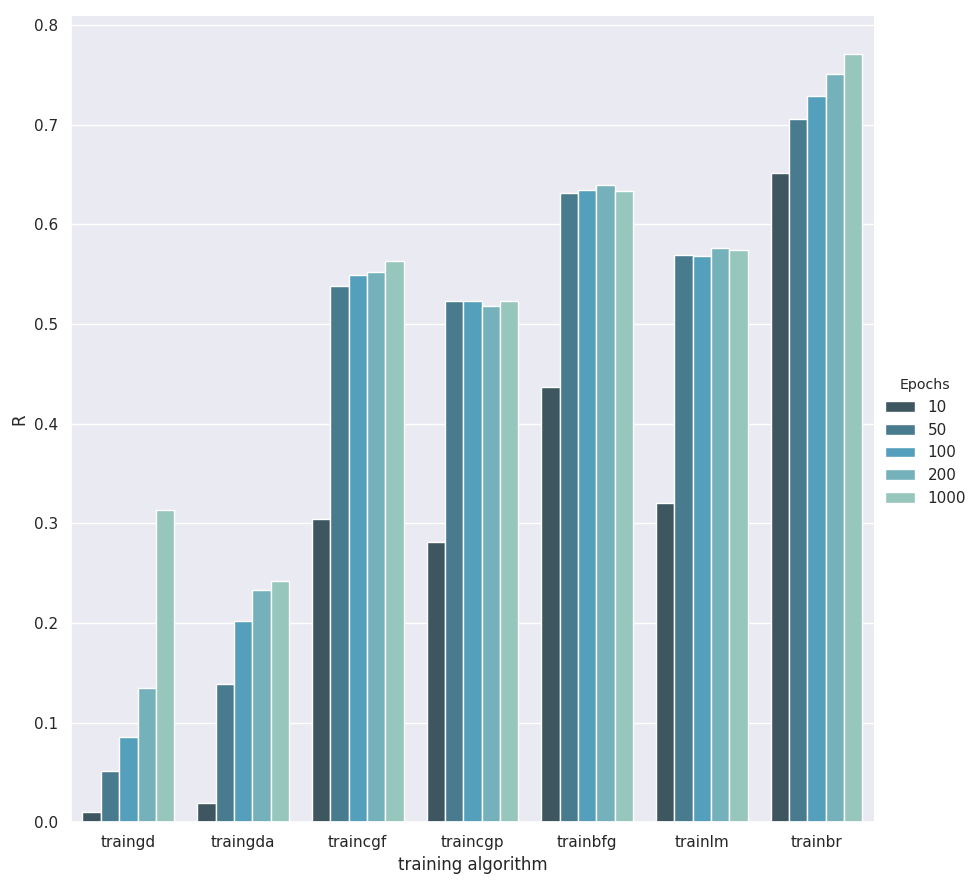
\includegraphics[width=\linewidth]{EpochsR}
%            \caption{Number of epochs - R}
%        \end{subfigure}
%        \begin{subfigure}{0.33\linewidth}
%            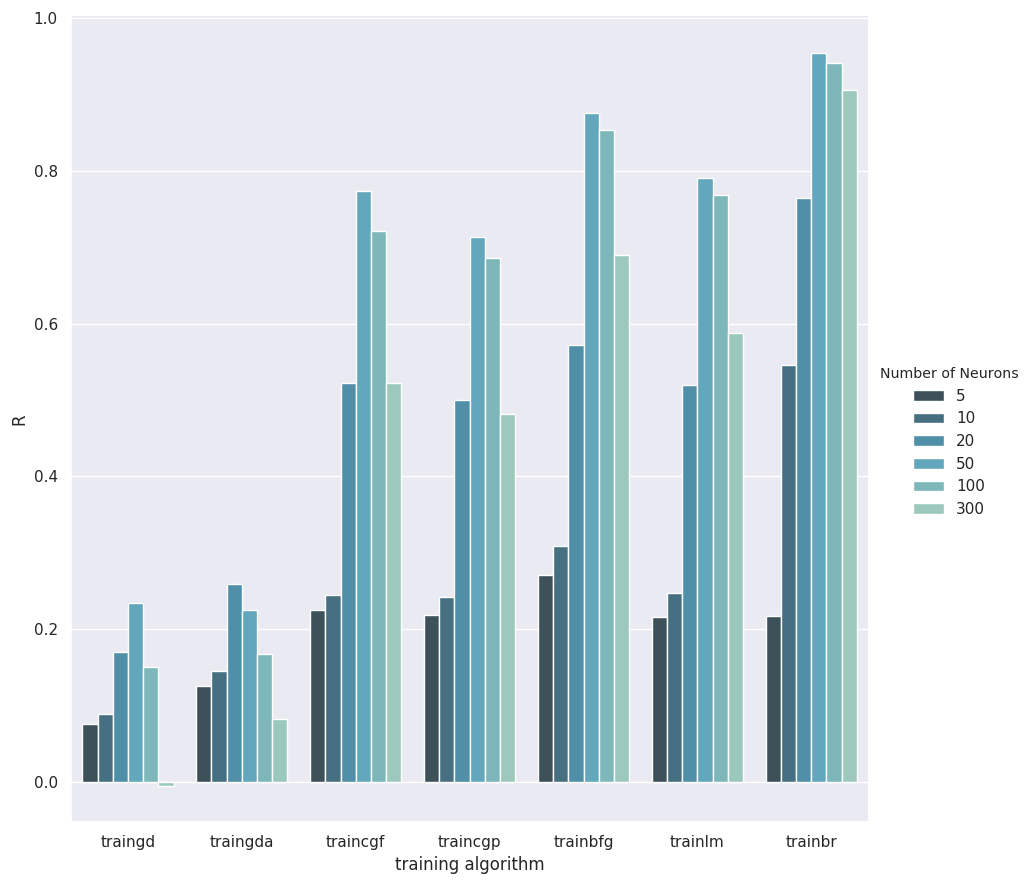
\includegraphics[width=\linewidth]{neuronsR}
%            \caption{Number of hidden neurons - R}
%        \end{subfigure}
%        \begin{subfigure}{0.33\linewidth}
%            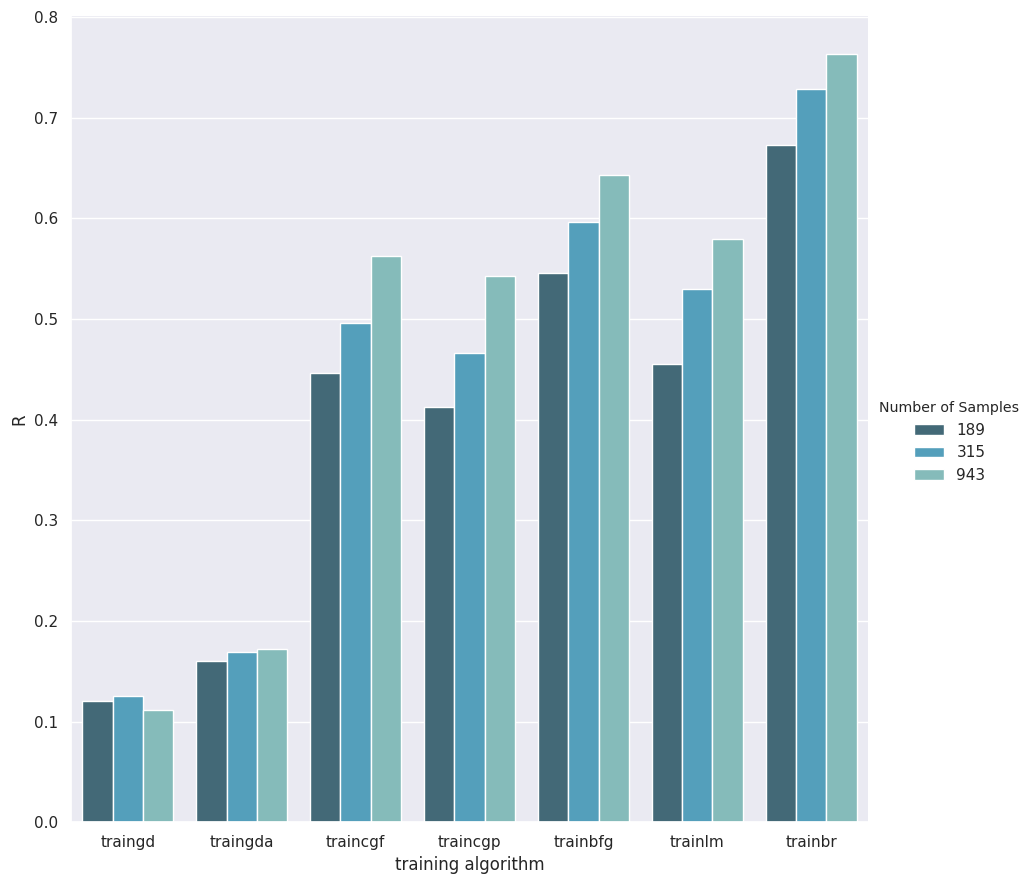
\includegraphics[width=\linewidth]{SamplesR}
%            \caption{Number of samples - R}
%        \end{subfigure}
%
%
%		\begin{subfigure}{0.33\linewidth}
%            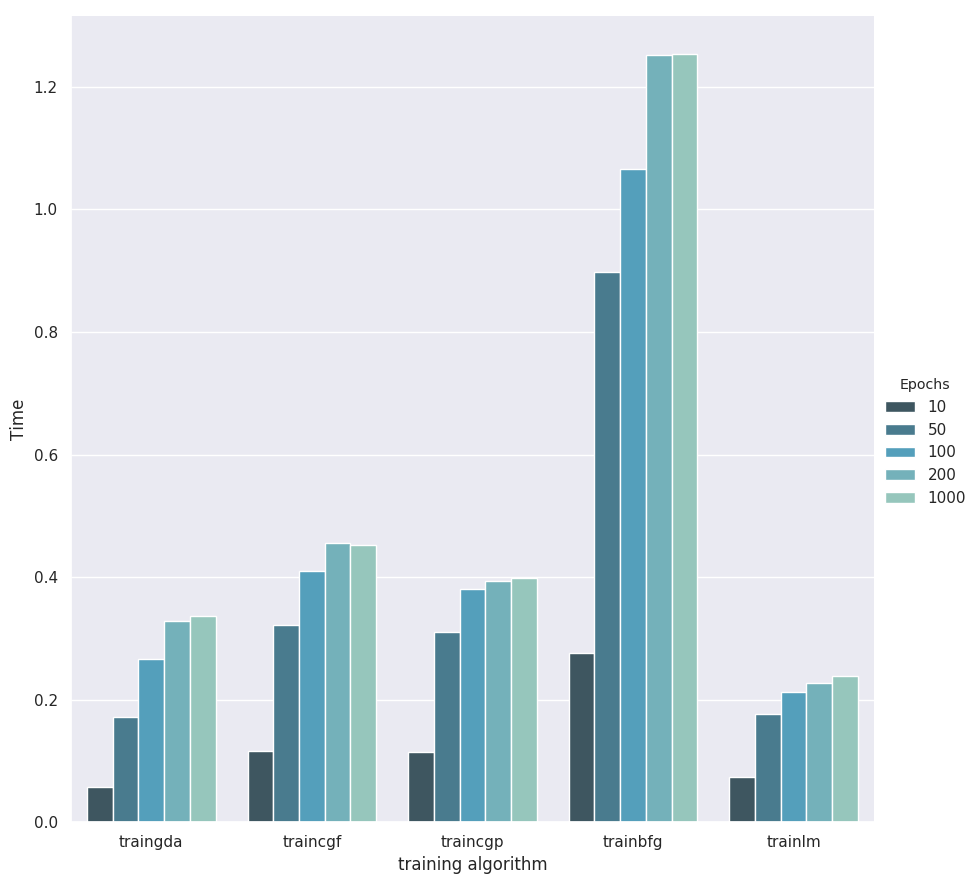
\includegraphics[width=\linewidth]{EpochsTime}
%            \caption{Number of epochs - Time}
%        \end{subfigure}
%        \begin{subfigure}{0.33\linewidth}
%            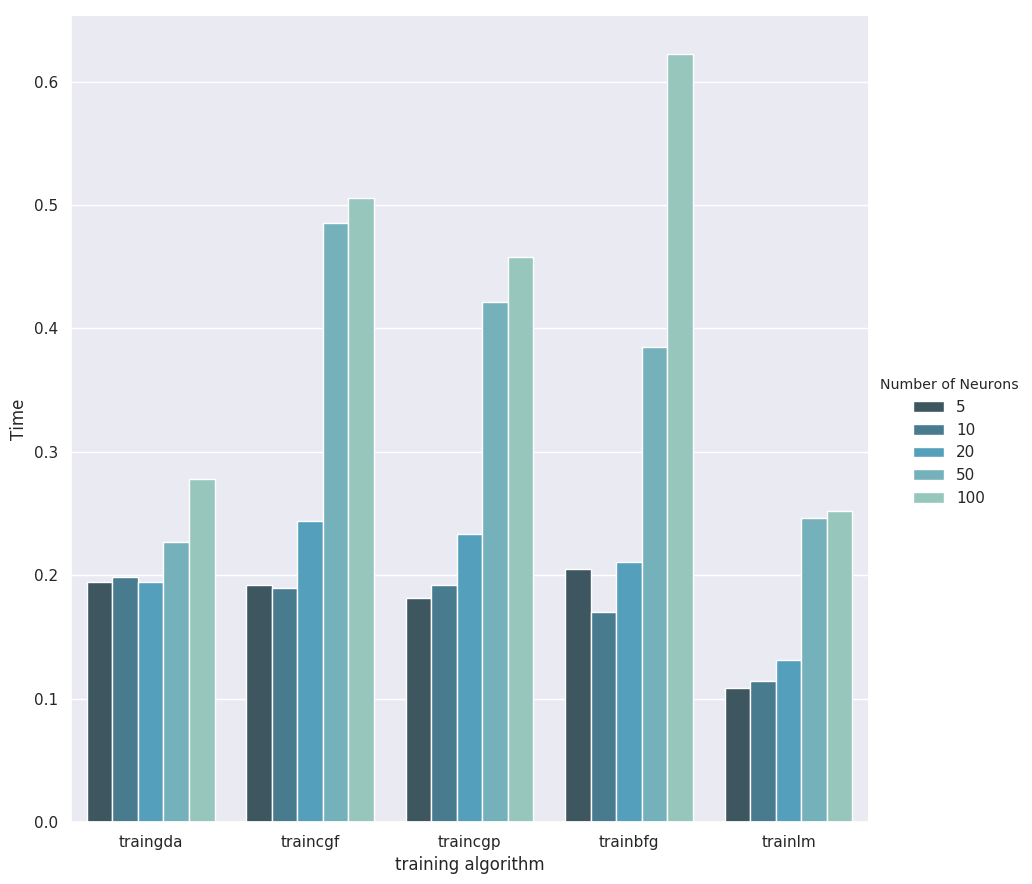
\includegraphics[width=\linewidth]{neuronsTime}
%            \caption{Number of hidden neurons - Time}
%        \end{subfigure}
%        \begin{subfigure}{0.33\linewidth}
%            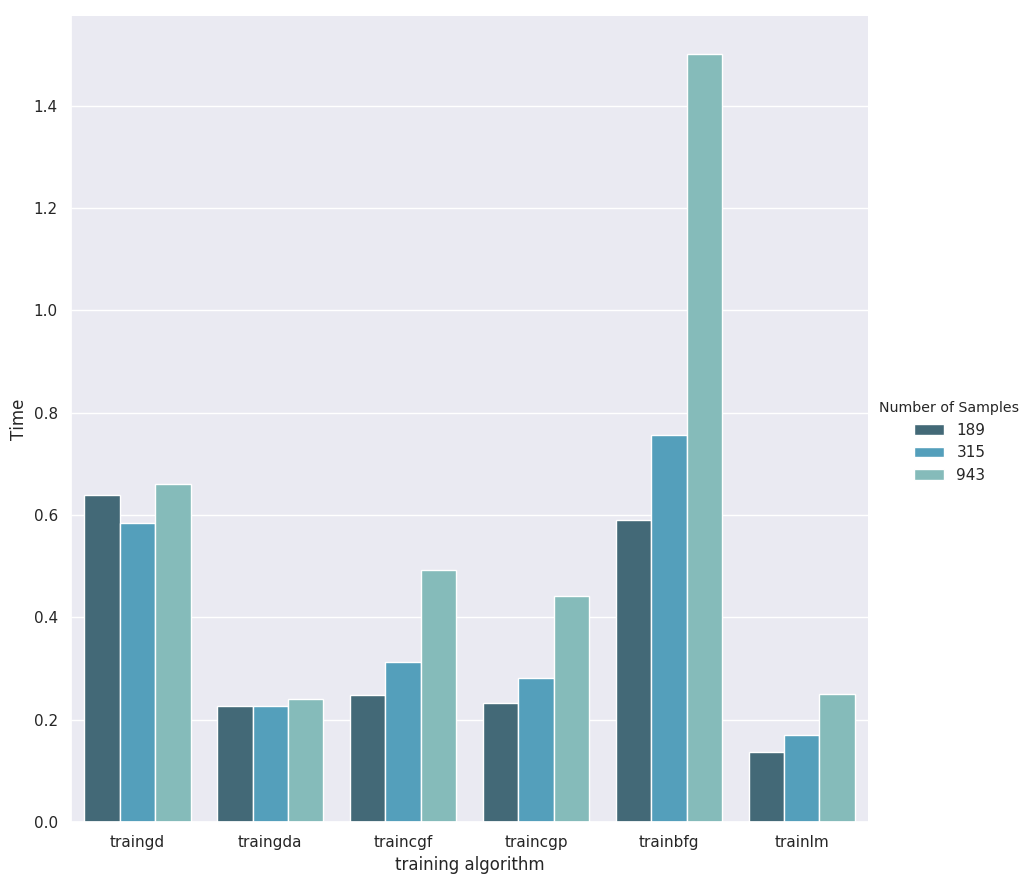
\includegraphics[width=\linewidth]{SamplesTime}
%            \caption{Number of samples - Time}
%        \end{subfigure}
%   
%        
%	
%        \caption{ Varying the effect of various parameters and measuring performance in terms of R value and training time.}        
%        
%                
%        
%        \label{fig:results}
%    \end{figure*}
%



\section{Exercise Session 1}

\subsection{A simple example: two Gaussians}


\textit{Obtain a line to classify the data by using what you know about the distributions of
the data. In which sense is it optimal?}

For a binary classification problem, the Bayes classification rule leads to a minimal probability of misclassification. According to Bayes rule, a test observation $x$ is assigned to a class $i^*$ so that $i^* = arg \max\limits_{i,\dots 2} P(C_i|x)$, where $P(C_i|x)$ denotes the posterior class probability of class $C_i$. This also corresponds to minimizing the overlap area between the distributions $P(C_1|x)P(C_1)$ and $P(C_2|x)P(C_2)$. If the data are generated from a Gaussian distribution with the same covariance matrix for the two classes, the optimal decision boundary is a linear seperating hyperplane which is independent of the overlap area between these Gaussian distributions. As a consequence, in the case of non-seperable classes with overlapping distributions, misclassifications should be tolerated.


\subsection{Support vector machine classifier}

\textit{What do you observe when you add more data points to the dataset - both
on the right and on the wrong side of the hyperplane. How does it affect the
classification hyperplane?}

Consider a given training set $\{x_k,y_k\}^N_{k=1}$ with input data $x_k \in \mathcal{R}^N $ and output data $y_k \in \mathcal{R} $ with class labels $y_k \in \{-1,+1 \}$. According to Vapnik's extension of linear Support Vector Machines (SVMs) to the non-seperable case, the optimization problem in its primal form becomes:

\begin{equation}
\min\limits_{w,b,\xi} J(w,b) = \frac{1}{2}w^Tw + c \sum_{k=1}^{N}\xi_k
\end{equation}
subject to
\begin{equation*}
\begin{cases}
\begin{aligned}
  y_k[w^Tx_k+b] \geq 1-\xi_k, k=1,...,N \\
  \xi_k \geq 0, k =1,...N
\end{aligned}
\end{cases}
\end{equation*}
where $\xi_k$ slack variables measure the distance of each data point $x_k$ from the marginal hyperplane. Slack variables allow a data point $x_k$ example to be in the margin ($0< \xi<1$), or to be misclassified ($\xi>1$).
The term $c \sum_{k=1}^{N}\xi_k$ is used to penalize misclassification and margin errors. Additions on the wrong side of the hyperplane drastically change the decision boundary as they increase the value of the penalization term, as opposed to additions on the correct side of the hyperplane that have a minor impact to the solution. This behaviour is illustrated in Figure~\ref{fig:adding}. 


    \begin{figure*}[]
        \begin{subfigure}{0.33\linewidth}
            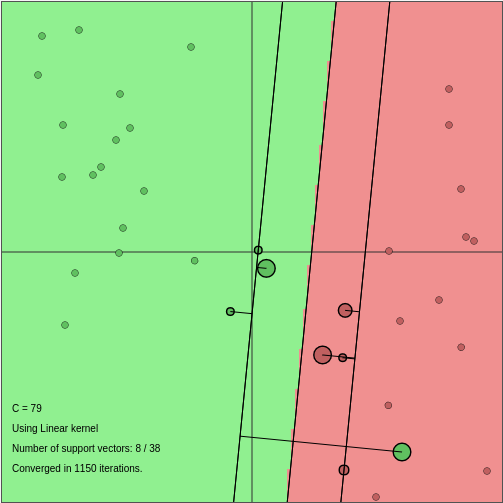
\includegraphics[width=\linewidth]{add1}
            \caption{original solution}
        \end{subfigure}
        \begin{subfigure}{0.33\linewidth}
            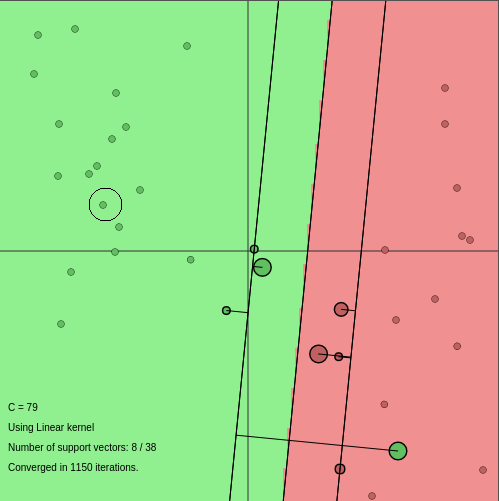
\includegraphics[width=\linewidth]{add2}
            \caption{new green data point on the right side}
        \end{subfigure}
        \begin{subfigure}{0.33\linewidth}
            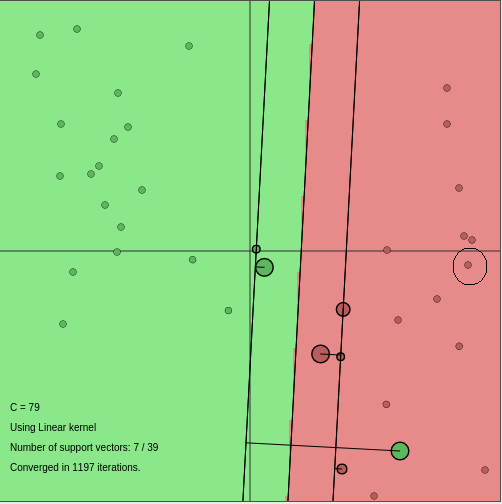
\includegraphics[width=\linewidth]{add3}
            \caption{new red data point on the right side}
        \end{subfigure}


		\begin{subfigure}{0.33\linewidth}
            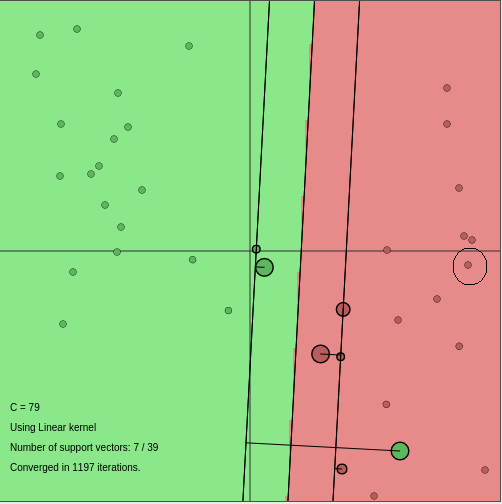
\includegraphics[width=\linewidth]{add3}
            \caption{original solution}
        \end{subfigure}
        \begin{subfigure}{0.33\linewidth}
            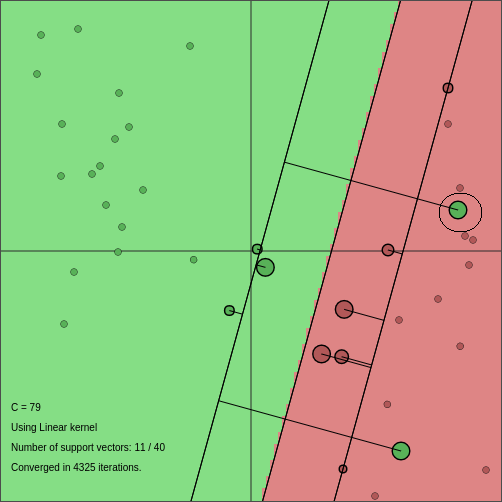
\includegraphics[width=\linewidth]{add4}
            \caption{new green data point on the wrong side}
        \end{subfigure}
        \begin{subfigure}{0.33\linewidth}
            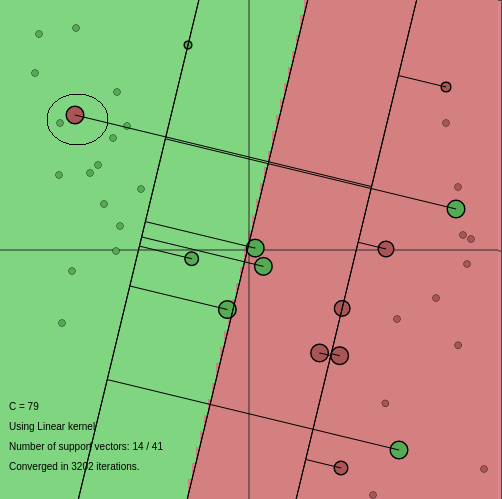
\includegraphics[width=\linewidth]{add5}
            \caption{new red data point on the wrong side}
        \end{subfigure}
   
        
	
        \caption{ Adding more points to the dataset on the right side of the hyperplane (first row) and on the wrong side of the hyperplane (second row). Adding points on the wrong side of the hyperplane drastically changes the hyperplane, as opposed to adding points on the right side of the plane which has a minor effect.}        
        
                
        
        \label{fig:adding}
    \end{figure*}



\textit{Try out different values of the regularization hyperparameter c and the kernel
parameter sigma. What is the role of the parameters? How do these parameters
affect the classification outcome?}

\begin{figure*}[]
        \begin{subfigure}{0.33\linewidth}
            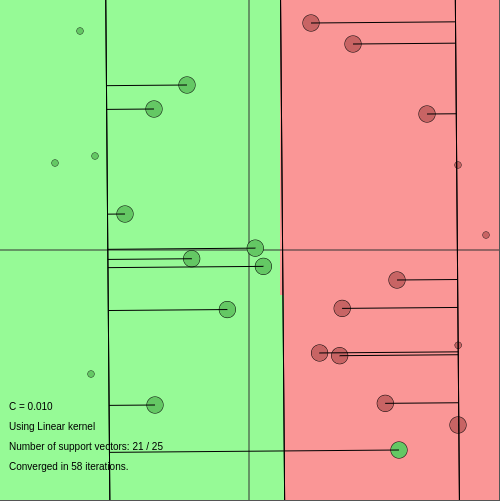
\includegraphics[width=\linewidth]{svmc01}
            \caption{c=0.1}
        \end{subfigure}
        \begin{subfigure}{0.33\linewidth}
            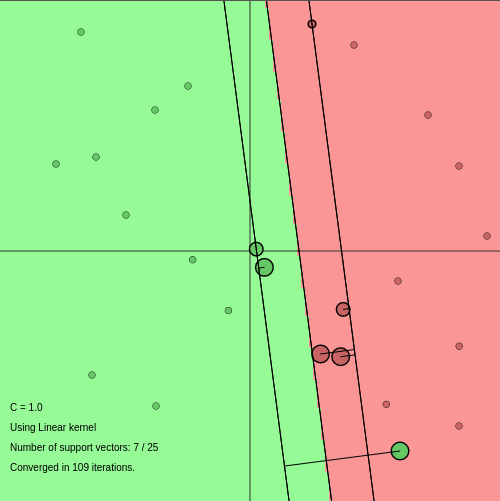
\includegraphics[width=\linewidth]{svmc10}
            \caption{c=1.0}
        \end{subfigure}
        \begin{subfigure}{0.33\linewidth}
            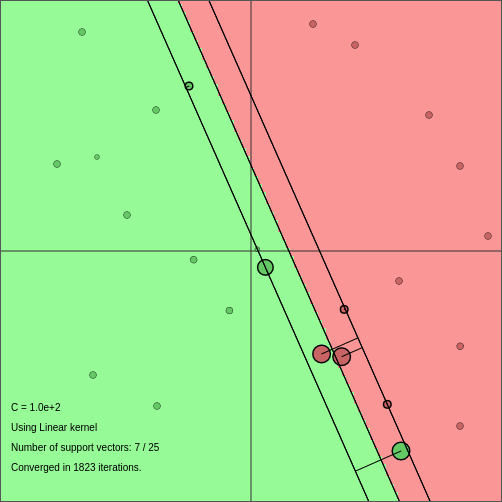
\includegraphics[width=\linewidth]{svmc100}
            \caption{c=100}
        \end{subfigure}



        \caption{Varying the $c$ parameter for the linear kernel. As c is increased from 0.1 (a) to 1.0 (b) and 100 (c) the hyperplane is adjusted and the margin becomes smaller as fewer misclassifications are tolerated.  }        
        
              
        \label{fig:c}
    \end{figure*}

The regularization hyperparameter c determines how much emphasis is put on maximizing the margin versus tolerating misclassification errors. For a large value of c, a large penality is assigned to misclassification/margin errors. A smaller value for c, allows to ignore points close to the boundary, and increases the margin. As c is increased, the hyperplane's orientation is changed, providing a much smaller margin. For the case of a linear kernel, this effect is illustrated in Figure~\ref{fig:c}. Indeed, higher values of $c$ produce a smaller margin and fewer support vector machines.

Kernel methods have been widely applied to support vector machines, as they allow to operate in a different feature space and construct non linear models. The optimization problem now becomes:

\begin{equation}
\min\limits_{w,b,\xi} J(w,b) = \frac{1}{2}w^Tw + c \sum_{k=1}^{N}\xi_k
\end{equation}
subject to
\begin{equation*}
\begin{cases}
\begin{aligned}
  y_k[w^T\phi(x_k)+b] \geq 1-\xi_k, k=1,...,N \\
  \xi_k \geq 0, k =1,...N
\end{aligned}
\end{cases}
\end{equation*}

where $\phi(x_k)$ can be infinite dimensional. By constructing the lagragian, one can solve the problem in its dual form:


\begin{equation}
\max\limits_{\alpha} J(w,b) = -\frac{1}{2}\sum_{k,l=1}^{N}y_ky_lK(x_k,x_l)\alpha_k\alpha_l +  \sum_{k=1}^{N}\alpha_k
\end{equation}
such that
\begin{equation*}
\begin{cases}
\begin{aligned}
   \sum_{k=1}^{N}\alpha_ky_k=0 \\
  0 \geq a_k \geq c, k =1,...N
\end{aligned}
\end{cases}
\end{equation*}

where $K(x_k,x_l)=\phi(x_k)^T\phi(x_l)$ is the kernel function. The idea behind kernel methods is that if the data is not separable in the original space they can become separable in a higher dimensional space. This is better illustrated in Figure~\ref{fig:example}, for the case of 1-dimensional data. In the left plot, the original data points are shown which are not linearly separable in this 1-dimensional space. After applying the transformation $\phi(x)=x^2$ a second dimension is added to the feature space and the classes become linearly separable.

The kernel trick allows to work in feature spaces without actually needing to perform any computations in this space. The beauty of kernel methods lies exactly in their ability to represent the data only through a set of pairwise similarity comparisons between the original data observations (by using their original coordinates in the lower dimensional space), instead of explicitly applying the transformations $\phi(x)$. Finally, in order to predict the class of a new test instance $x$ with a SVM classifier, a linear combination of kernel evaluations between the test instance and all the non-zero lagragian $\alpha$ variables should be computed:
  

\begin{equation}
y(x) = sign[\sum_{k=1}^{N}\alpha_ky_kK(x,x_k) +b ]
\end{equation}

We are particularly interested in the Gaussian (RBF) kernel:
\begin{equation}
K(x,x_k) = exp(-\frac{||x-x_k||^2_2}{\sigma^2})
\end{equation}

The Gaussian kernel measures the similarity between the test instance $x$ and any training instance $x_k$ as a function of the Euclidean distance. Since $e^{-x}$ is a monotonically decreasing function, the higher the value of the term $\frac{||x-x_k||^2_2}{\sigma^2}$, the smaller $K(x,x_k)$ will be. If the distance between $x$ and $x_k$ is much larger than sigma, the kernel function tends to be closer to zero. With the use of Gaussian kernel, each training data point shapes a covering sphere around its center that subject to the width of $\sigma$. This effect is illustrated clearly in Figure~\ref{fig:rbf} (e-g). Whenever the distance from a training instance exceeds this radius $\sigma$, the kernel value of this instance will get below the threshold value and its effect will vanish. Thus, if $\sigma$ is very small, the data points will tend to be too dissimilar which can lead to over-fitting. In other words, smaller values for $\sigma$ will tend to construct a classifier centered around local areas  while larger values will produce the opposite effect. On the other hand, if $\sigma$ is very large, the data points will tend to be very similar and under-fitting can arise. 

\begin{figure}[]

            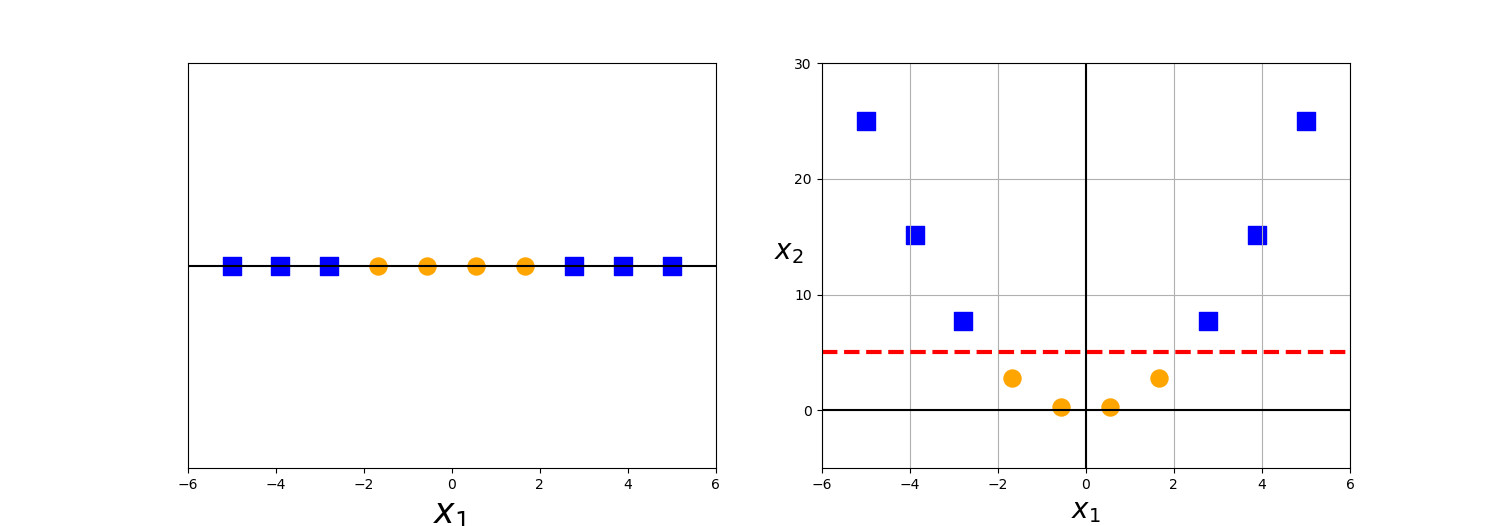
\includegraphics[width=\linewidth]{example}
      
        \caption{ In the left plot, the original data points are shown which are not linearly separable in the 1-dimensional space. After applying the transformation $\phi(x)=x^2$ a second dimension is added to the feature space and the classes become linearly separable }        
        
              
        \label{fig:example}
    \end{figure}

Some observations are summarized below:

\begin{itemize}  
\item For any given $c$, as $\sigma \to \infty$ the resulting classifier behaves like a linear classifier. Figure~\ref{fig:rbf} (e-h) shows this effect as the classification boundaries become more and more linear as $s$ is increased.
\item Under-fitting (all the data points are assigned the majority class) seems to occur in cases where $\sigma$ is fixed and $c \to 0$ or $\sigma \to 0$ and $c$ is fixed to a small value. Figure~\ref{fig:rbf} (a) illustrates a case of underfitting with a small $c$ and fixed $\sigma$.
\item Over-fitting (areas around the training data points of the minority class are classified as this class while the rest is classified as the majority class) occurs when $\sigma^2 \to 0$ and $c$ is fixed to a large value. This case is illustrated in Figure~\ref{fig:c} (e).

\end{itemize}


\begin{figure*}
% first row: 3 subfigures
\begin{subfigure}{0.3\textwidth}
   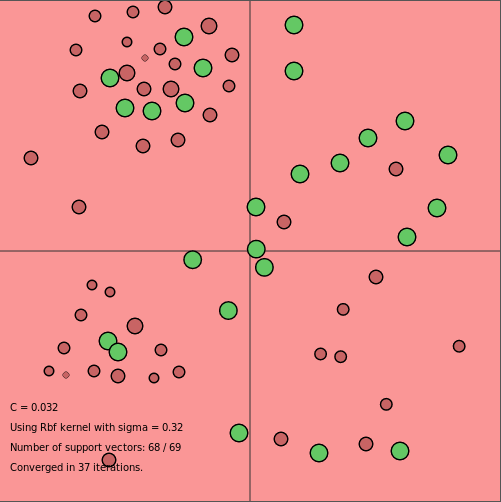
\includegraphics[width=\linewidth]{c=0032_s=032}
   \caption{$c=0.032, s=0.32$} \label{fig:x_a}
\end{subfigure}
\hspace*{\fill}
\begin{subfigure}{0.3\textwidth}
   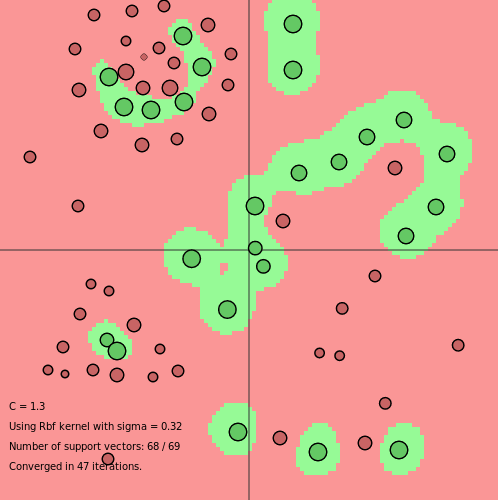
\includegraphics[width=\linewidth]{c=13_s=032}
   \caption{$c=1.3, s=0.32$} \label{fig:x_b}
\end{subfigure}
\hspace*{\fill}
\begin{subfigure}{0.3\textwidth}
   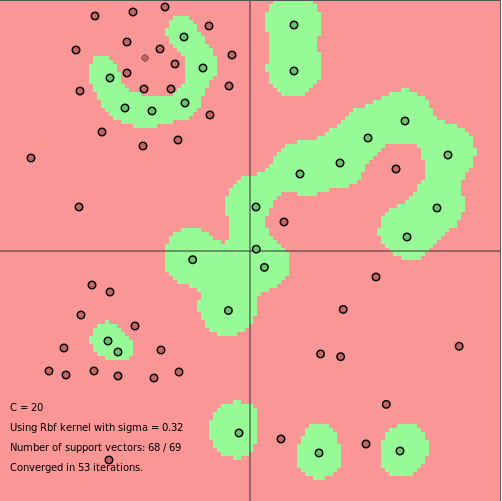
\includegraphics[width=\linewidth]{c=20_s=032}
   \caption{$c=20, s=0.32$} \label{fig:x_c}
\end{subfigure}

% 2nd row: 3 more subfigures
\bigskip
\begin{subfigure}{0.3\textwidth}
   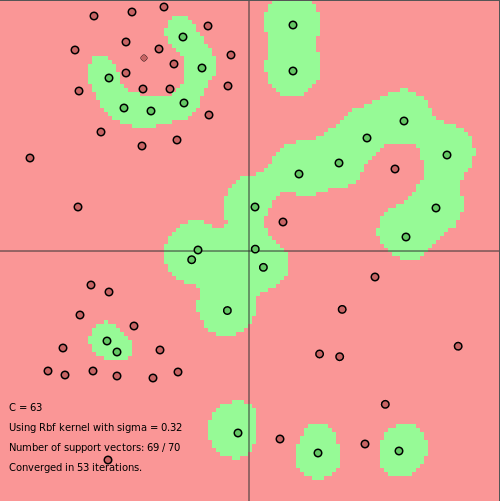
\includegraphics[width=\linewidth]{c=63_s=032}
   \caption{$c=63, s=0.32$} \label{fig:x_d}
\end{subfigure}
\hspace*{\fill}
\begin{subfigure}{0.3\textwidth}
   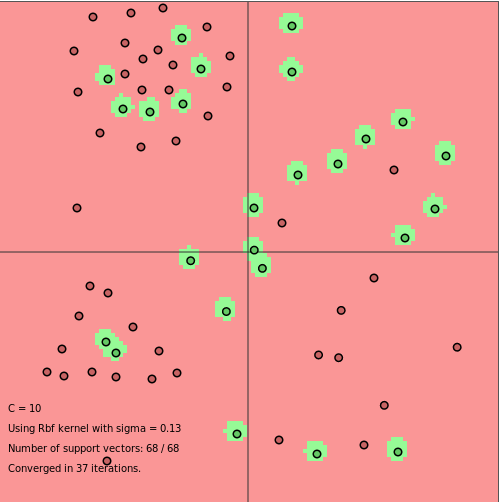
\includegraphics[width=\linewidth]{c_10_s013}
   \caption{$c=10, s=0.13$} \label{fig:x_e}
\end{subfigure}
\hspace*{\fill}
\begin{subfigure}{0.3\textwidth}
   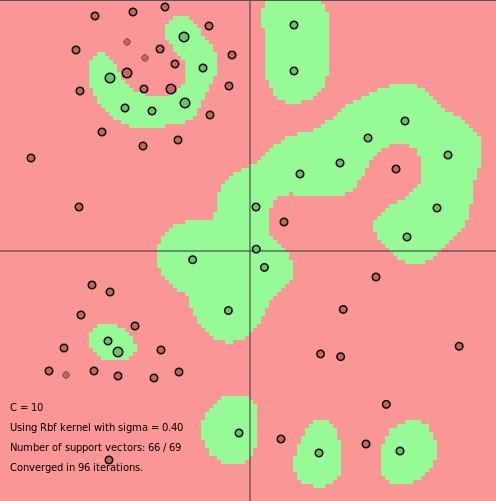
\includegraphics[width=\linewidth]{c=10_s=040}
   \caption{$c=20, s=0.43$} \label{fig:x_f}
\end{subfigure}

% 3rd row: just 2 subfigures, centered
\bigskip
\hspace*{\fill}
\begin{subfigure}{0.3\textwidth}
   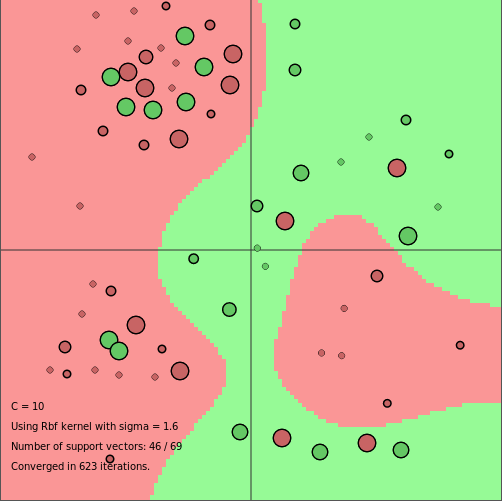
\includegraphics[width=\linewidth]{c=10_s=16}
   \caption{$c=10, s=1.6$} \label{fig:x_g}
\end{subfigure}%
\hspace*{0.05\textwidth}%
\begin{subfigure}{0.3\textwidth}
   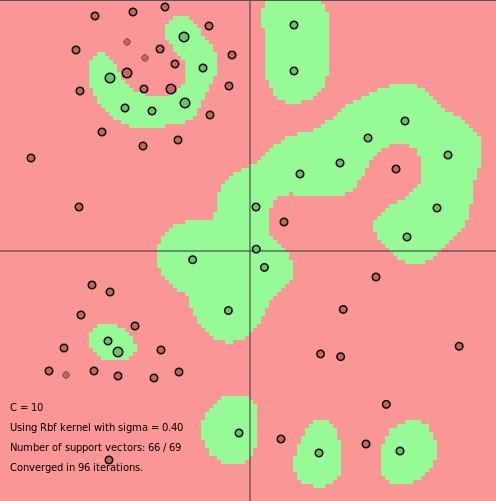
\includegraphics[width=\linewidth]{c=10_s=040}
   \caption{$c=10, s=20$} \label{fig:x_h}
\end{subfigure}
\hspace*{\fill}

\caption{Varying $c$ and $\sigma$ for the RBF kernel. }
\end{figure*}

    \label{fig:rbf}

\begin{figure}[]
        \begin{subfigure}{0.450\linewidth}
            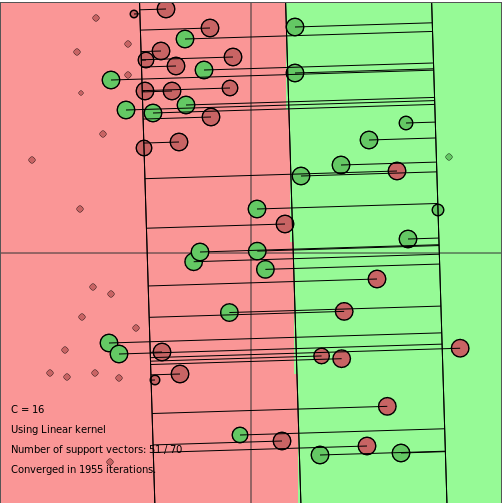
\includegraphics[width=\linewidth]{linear}
            \caption{Linear kernel}
        \end{subfigure}
        \begin{subfigure}{0.45\linewidth}
            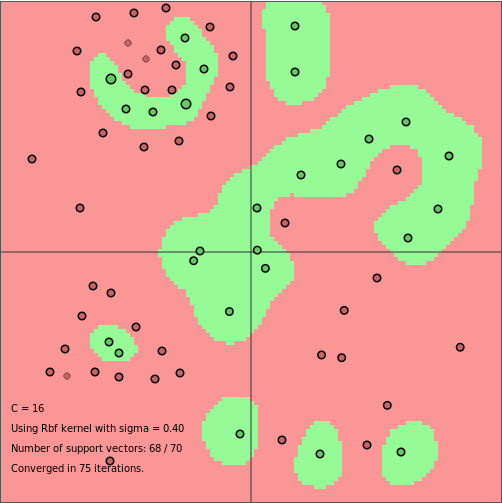
\includegraphics[width=\linewidth]{rbf}
            \caption{RBF kernel}
        \end{subfigure}
       

        \caption{Comparison of the decision surfaces produced by a linear (a) and an RBF (b) kernel. }        
        
              
        \label{fig:compare}
    \end{figure}



\textit{Compare classification using the linear kernel with classification using the RBF kernel.
Which performs better? Why?}

 Figure~\ref{fig:compare} shows the result of applying a linear and a Gaussian kernel for the same set of training data points. Clearly, the Gaussian kernel performs better since it is able to produce non-linear decision boundaries. The linear kernel is not able to produce


\textit{What is a support vector? When does a particular datapoint become a support vector?
When does the importance of the support vector change? Illustrate visually. Note that
a support vector is indicated by a large circle with bold-lined circumference and that
its importance is proportional to the size in the online application.}

A property of the SVM is that the solution vector is sparse, which means that many of the resulting $a_k$ values of equation (4) will be zero. The  sum $\sum_{k=1}^{\#SV}\alpha_ky_kK(x,x_k)$ will therefore be computed only over the non zero $a_k$ values instead of all the training data points. The training data points corresponding to non-zero $a_k$ values are called support vectors and are located close to the decision boundary.


\subsection{
Least-squares support vector machine classifier}

\subsubsection{
Influence of hyperparameters and kernel parameters}
%The RBF kernel, defined as $k(x,x^')=exp(-\gamma||x-x^'||^2$ the $\sigma$ %parameter also has a significant effect on the decision boundary.


\textit{Try out a polynomial kernel with degree = 1, 2, 3, . . . and t = 1 (fix gam = 1). Assess
the performance on the test set. What happens when you change the degree of the
polynomial kernel?}


In this exercise, the objective is to classify the Iris dataset and explore the effect of using different kernel functions. The training set consists of a set of 100 data points $\{x_k,y_k\}^{100}_{k=1}$ with input data $x_k \in \mathcal{R}^2 $ and output data $y_k \in \mathcal{R} $. The test set consists of 10 different data points.

For degree-d polynomials, the polynomial kernel is defined as:


\begin{equation}
K(x,x_k) = (x^Tx_k +\tau)^d
\end{equation}

where $d$ defines the degree of the polynomial kernel. According to the Mercer theorem, the only condition for the Kernel function $K$ is that it should be positive semi-definite. In that case, the convex nature of the dual SVM formulation problem guarantees that the solution found is going to be a global solution. The Mercer condition holds for all $\sigma$ values in the RBF kernel as expressed in equation 5 and positive $\tau$ values in the polynomial kernel as described in equation 6.

%A polynomial kernel $K(x,x_k) = (x^Tx_k)^d$ is equivalent to a polynomial basis expansion, with all terms of order d. It should be noted that computing a polynomial basis expansion requires $O(n^d)$ time while computing a polynomial kernel requires $O(n)$ time. By including $\tau$ in the equation $K(x,x_k) = (x^Tx_k +\tau)^d$ the result is that the low-order parts of the polynomial expansion tend to have a larger impact.


As most practical questions in machine learning, the choice of the kernel parameters is data dependent. The typical procedure is to first train a linear kernel first and observe if performance is improved by using non linear kernels. 
The degree parameter controls the flexibility of the decision boundary. Higher degree kernels yield a more flexible decision boundary but also increase the risk of overfitting. As more and more parameters are added to the model, the complexity increases which in turn leads to models of low bias but high variance.

Figure~\ref{fig:iris} shows the decision boundary obtained for a linear kernel (a) and polynomial kernels of degree 2-4 (b-d). For the linear kernel, the classification error is 55\% (e.g. 11 out of 20 observations are misclassified). Applying a quadratic kernel significantly improves the performance as the prediction error drops to 5\%. For polynomials of degree $\geq 3$ the prediction error drops to 0. In the case of high order polynomial kernels the decision boundaries become more and more complex which may lead to overfitting. This is illustrated in Figure 6 (e) and (f) where a polynomial kernel of degree 15 and 20 are applied. The prediction errors for the 15 degree and 20 cases are 5\% and 20\% respectively. To conclude, following the Occam’s razor principle, the polynomial with the lowest degree that performs best should be chosen. In this particular example, the ideal choice would be either a quadratic or a cubic polynomial since the prediction error is already very small or zero.

As more and more parameters are added to a model, the complexity of the model rises and variance becomes our primary concern while bias steadily falls


\textit{Let’s now focus on the RBF kernel with squared kernel bandwidth $\sigma^2$. \\
-Try out a good range of different sig2 values as kernel parameters (fix gam = 1).
Assess the performance on the test set. What is a good range for sig2?\\
-Fix a reasonable choice for the sig2 parameter and compare the performance
using a range of gam. What is a good range for gam?}


Values for parameters $\gamma=$ and $\sigma^2$ are varied from 0.01 to 100 and performance on the test set is assessed and presented in Figure~\ref{fig:cgama}. The optimal values are where the prediction error is close to 0. For $\sigma^2 \in [0.05,5] $, the parameter $\gamma$ can be set to $\gamma \in [0.5,10] $ and achieve an accurate classification result with a prediction error of 0. Another possible range of values is 
$\sigma^2 \in [0.5,5], \gamma \in [50,100]$. As previously mentioned, a small error for $\gamma$ allows to ignore points close to the boundary and increases the margin, resulting in tolerating more errors.
An overestimated value value for $\sigma$ raises the prediction error 
since the exponential in equation 5 will behave almost linearly and the higher-dimensional projection will lose its non-linear discriminative power. On the other hand, if underestimated, the decision boundary will become highly sensitive to noise as the model will start to overfit the data. In the next subsection, 
automated tuning algorithms for hyperparameter optimization are explored.


\begin{figure}[]

            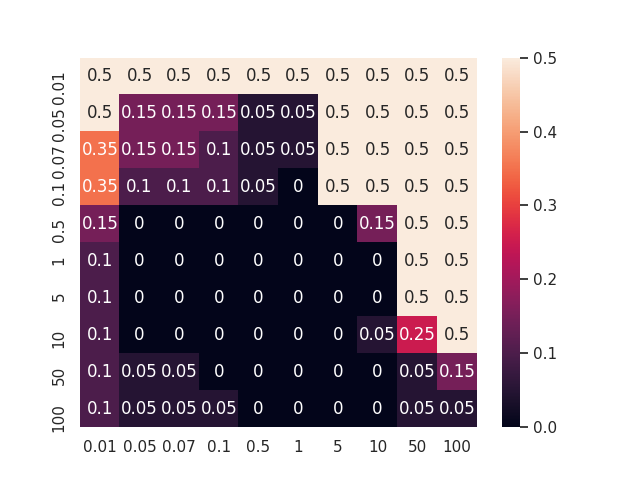
\includegraphics[width=\linewidth]{cgama}
      
        \caption{ Prediction error on the test set is measured for a different range of values for $\sigma$ (x-axis) and $\gamma$ (y-axis). The figure suggests that a possible range of values for the two parameters is $\sigma \in [0.05,5], \gamma \in [1,10]$.   }        
        
              
        \label{fig:cgama}
    \end{figure}





    \begin{figure*}[]
        \begin{subfigure}{0.33\linewidth}
            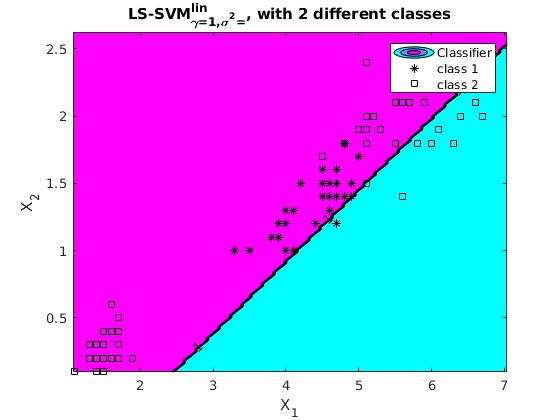
\includegraphics[width=\linewidth]{iris_linear}
            \caption{Polynomial of degree 1. Prediction error: 55\%}
        \end{subfigure}
        \begin{subfigure}{0.33\linewidth}
            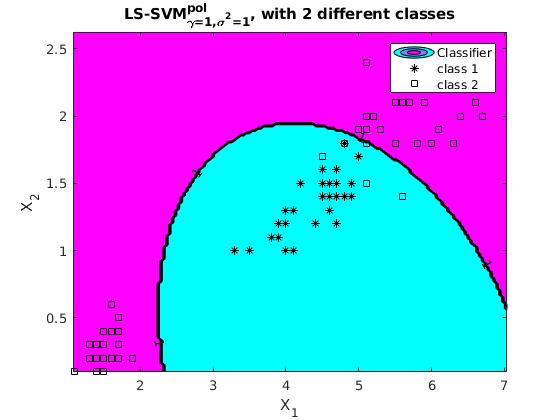
\includegraphics[width=\linewidth]{iris_degree2}
            \caption{degree 2.
Prediction error: 5\%}
        \end{subfigure}
        \begin{subfigure}{0.33\linewidth}
            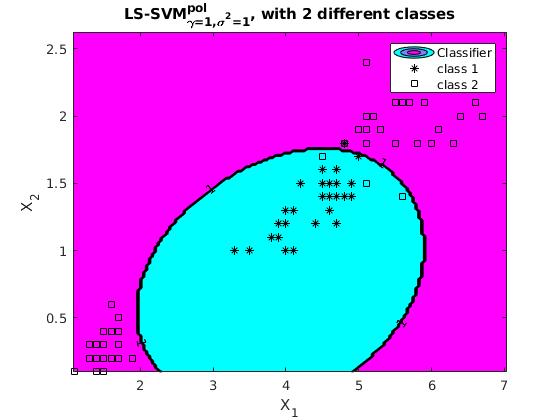
\includegraphics[width=\linewidth]{iris_degree3}
            \caption{degree 3.
Prediction error: 0\%}
        \end{subfigure}


		\begin{subfigure}{0.33\linewidth}
            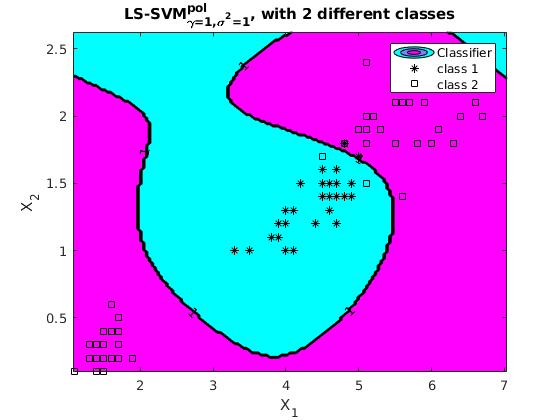
\includegraphics[width=\linewidth]{iris_degree4}
            \caption{degree 4.
Prediction error: 0\%}
        \end{subfigure}
        \begin{subfigure}{0.33\linewidth}
            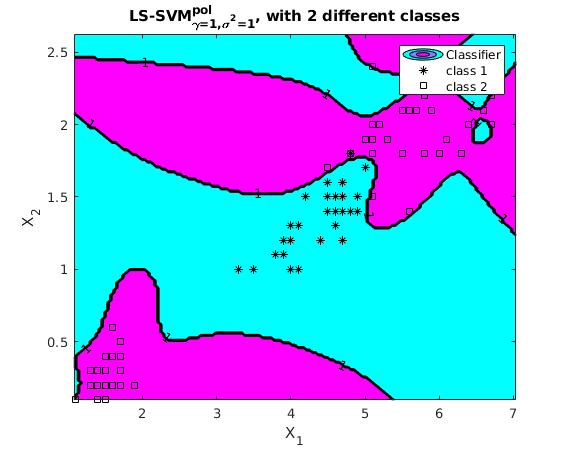
\includegraphics[width=\linewidth]{iris_degree_15}
            \caption{degree 15.
Prediction error: 5\%}
        \end{subfigure}
        \begin{subfigure}{0.33\linewidth}
            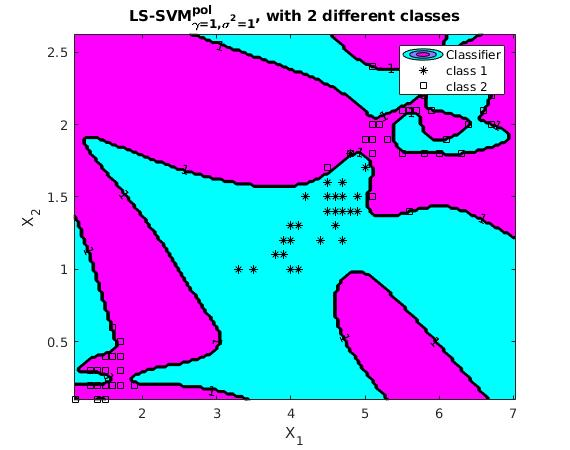
\includegraphics[width=\linewidth]{iris_degree_20}
            \caption{degree 20.
Prediction error: 20\%}
        \end{subfigure}
   
        
	
        \caption{ Varying the degree of the polynomial kernel. A linear kernel is unable to properly separate the data points. Increasing the degree of the polynomial kernel results in more expressive decision surfaces. However, if the degree of the polynomial kernel is too high this results in overfitting.}        
        \label{fig:iris}
    \end{figure*}
    
   

    \begin{figure*}[]
        \begin{subfigure}{0.50\linewidth}
            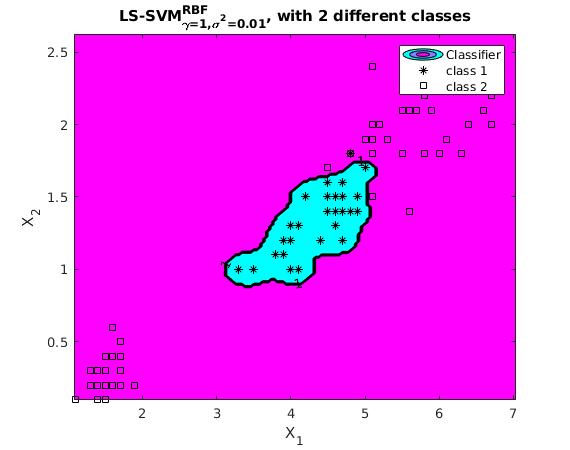
\includegraphics[width=\linewidth]{RBFgam1sig001}
            \caption{$\gamma=1, \sigma=0.01$}
        \end{subfigure}
        \begin{subfigure}{0.50\linewidth}
            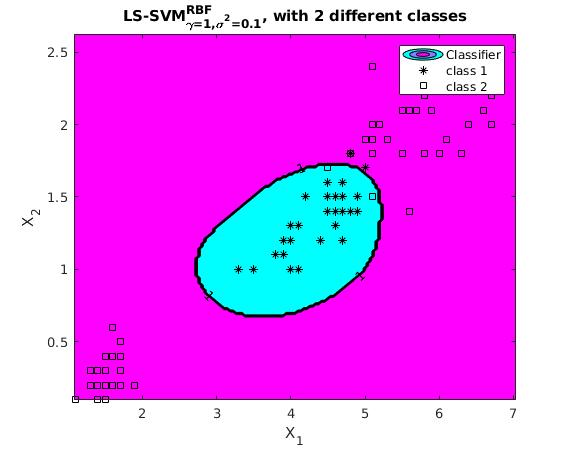
\includegraphics[width=\linewidth]{RBFgam1sig01}
            \caption{$\gamma=1, \sigma=0.1$}
        \end{subfigure}
        \begin{subfigure}{0.50\linewidth}
            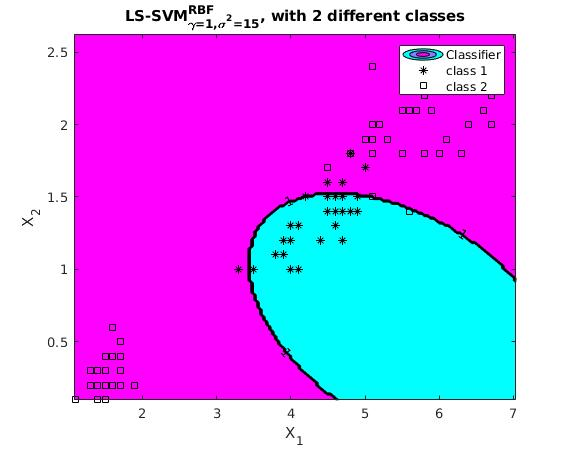
\includegraphics[width=\linewidth]{RBFgam1sig15}
            \caption{$\gamma=1, \sigma=15$}
        \end{subfigure}
           \begin{subfigure}{0.50\linewidth}
            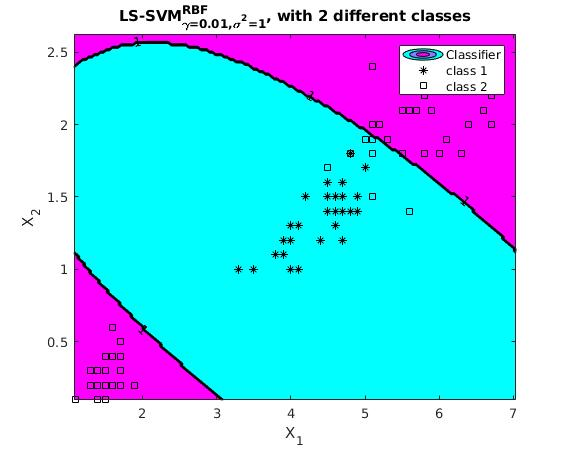
\includegraphics[width=\linewidth]{RBFsigma1gamma001}
            \caption{$\gamma=0.01, \sigma=1$}
        \end{subfigure}
   
        \caption{Varying $\sigma$ and $\gamma$ parameters in the RBF kernel. In (a) the decision boundary is centered around the points of one class which impacts the generalization ability of the classifier. In (d)  }                 
        
        \label{fig:irisrbf}
    \end{figure*}



\subsubsection{Tuning parameters using validation}

\textit{Compute the performance for a range of gam and sig2 values (e.g., $\gamma$, $\sigma^2$ = 10 −3 ,
. . . , 10 3). Use the random split method, 10-fold crossvalidation and leave-one-out
validation. Visualize the results of each method: do you observe differences? Interpret
the results: which values of gam and sig2 would you choose?}



In the previous question, it was shown that the performance of the solution provided by a Least-squares support vector machine classifier depends on the choice of both the $\gamma$ parameter and the parameters related to the kernel function (e.g. $d$ in equation 6 and $\sigma$ in equation 5). The goal of this exercise is to examine the efficiency and measure the performance of three different automatic tuning methods that split the raining data into a training and a validation set. Figure~\ref{fig:val} shows the contour plots that describe the performance for each one of the three methods.

\textbf{Random Split} Random Split is the simplest approach to fine-tune different parameters. The training dataset is randomly split into a training and a validation set and the model is evaluated in the latter.
Since the validation set includes data independent of that used for training, the performance of the validation set reflects the generalization ability of the model and the choice of different parameters can experimentally be tested. The validation set should not be confused with the test set which is meant to assess the performance of a fully-specified model. The error on the test set provides an unbiased estimate of the generalization error, assuming that the test set is representative of the population and follows the same probability distribution as the training set.

The main problem with the random split method is that it does not exploit the full set of data to train the model which may be problematic in cases where the size of the available data is small. The generalization error will depend on the split and different validation splits may give a different generalization errors. This means that the error estimates will be highly biased, resulting in a possibly large difference between the true test error and the estimated test error. The model will also has a high variance since it becomes very sensitive to the particular choice of data over which it is evaluated. 





\textbf{k-fold Cross Validation}

In $k$-fold cross validation, the original data is randomly partitioned into $k$ subsets of equal size. A single subset is used as a validation set and the model is trained on the remaining $k-1$ subsets. This process is repeated $k$ times, with a different $k$ subset used as a validation set each time. The obtained $k$ results are averaged and a single estimation is produced to evaluate the performance.

The $k$-fold cross validation method tries to overcome the bias induced by the random split method. If the mean performance is satisfying this means that the model gives low error on average, ensuring that the model's notions about the data should be accurate. On the other hand, examining the standard deviation of the errors can provide an insight about the model's variance. If the standard deviation of the errors is high, this means that the model's performance varies a lot with the different splits. The main advantage of this method mainly comes from using the whole training set, providing a statistical generalization of the the random split method.

The number of folds should allow the size of each of the validation sets to be large enough to accurately reflect the population. Some observations on the size of $k$ are summarized below:

\begin{itemize}

\item A large value of $k$ will result in a small bias of the error estimates and a higher variance.
\item A small $k$ will result in a high bias in the error estimates and in a lower variance


\end{itemize}





\textbf{Leave-one-out validation} Leave-one-out cross-validation is $k$-fold cross validation applied to its logical extreme, with the parameter $k$ being equal to the number of available training instances $N$. The model is trained $N$ separate times on all the available data except one observation which is used for test. The performance is estimated by averaging the errors and models are evaluated the same way as before.

 It is interesting to observe that the predictions made by the models on each leave-one-out fold will have less variability since the training set is almost the same each time (the full dataset minus one data point). Intuitively, the leave-one-out method provides has a lower bias compared to $k$-fold validation since almost all of the available data are used for training.  The main drawback of this method is its computational complexity. For a training set that includes $p$ examples, leave-one-out validation requires training the model $p$ times which may become a problem for large datasets.



\begin{figure*}
% first row: 3 subfigures
\begin{subfigure}{0.3\textwidth}
   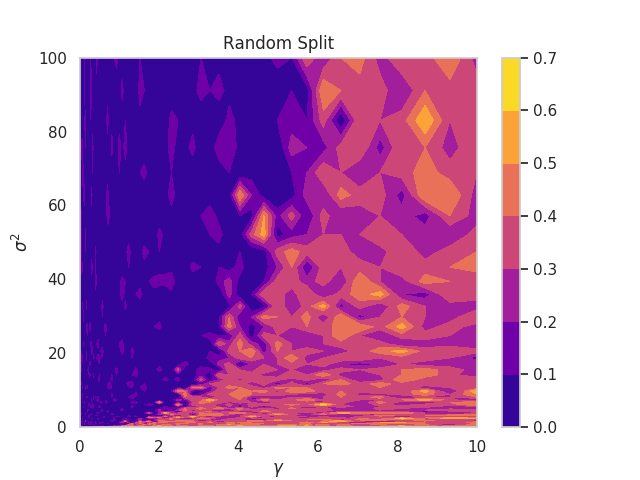
\includegraphics[width=6.6cm]{randomsplit}
   \caption{Random split} \label{fig:x_a}
\end{subfigure}
\hspace*{\fill}
\begin{subfigure}{0.3\textwidth}
   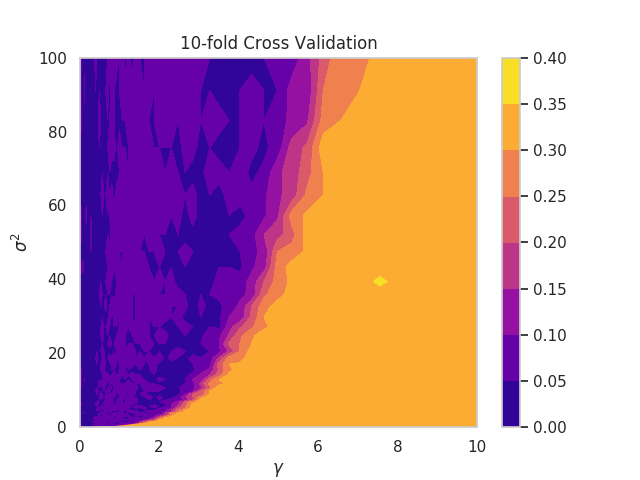
\includegraphics[width=6.6cm]{10fold}
   \caption{10-fold cross validation} \label{fig:x_b}
\end{subfigure}
\hspace*{\fill}
\begin{subfigure}{0.3\textwidth}
   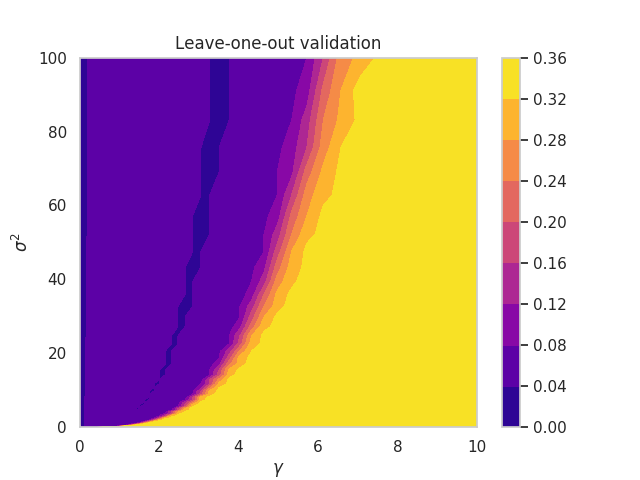
\includegraphics[width=6.6cm]{leaveone}
   \caption{leave-one-out cross validation } \label{fig:x_c}
\end{subfigure}


\caption{Visualization of the of misclassification error as a function of parameters $\sigma^2$ and $\gamma$ for Random split, 10-fold validation and leave-one-out validation }
 \label{fig:val}
\end{figure*}



\subsubsection{Automatic parameter tuning}
\textit{Try out the different 'algorithm'. What differences do you observe? Why do the
obtained hyperparameters differ a lot in different runs? What about the cost? Computational speed? Explain the results.}

Direct Search methods are optimization methods that do not use derivatives approximations. Instead, they sample the objective function at a finite number of points in each iteration and decide on which actions to perform based on these values. In this section, two different approaches for automatic parameter tuning are tested and compared: Nelder–Mead method and a grid search method.  The Nelder–Mead method is a heuristic search method that belongs to direct search optimization techniques and is often applied to nonlinear problems. The grid search works by evaluating all the different values for the parameters to be tuned within a certain range. Table~\ref{fig:tune1} summarizes the tuning results. The obtained hyperparameters differ every time the tuning is performed since the objective function is not convex and multiple minimum solutions may exist.

 

 First, the suitable starting points are determined using Coupled Simulated Annealing (CSA) and then the starting points are passed to the selected optimization algorithm.


 %The LS-SVMlab toolbox integrates three optimization algorithms: Nelder-Mead algorithm, Brute force Gridsearch and Line Search.



\begin{table*}\centering
\ra{1.3}
\begin{tabular}{@{}rrrrrrrccrrrcrrr@{}}\toprule
& \multicolumn{4}{c}{Nelder-Mead method} & \phantom{abc}& \multicolumn{2}{c}{Brute Force Gridsearch} &
\phantom{abc} \\
\cmidrule{2-5} \cmidrule{7-9} \cmidrule{10-12}
& $\gamma$ & $\sigma^2$ &     cost\% &&  $\gamma$ & $\sigma^2$ &    cost\% \\ \midrule
CSA\\
 &  6.0623 & 1.2143 &  0.0400 && 0.1930 & 5.49 & 0.04 \\

RDS\\
 &   1.4513 & 5.7490& 0.04 &&  0.0674 & 0.57 &0.03 && \\



\bottomrule
\end{tabular}
\caption{Hyperparameters tuned with Nelder-Mead method and Brute Force Gridsearch }
       \label{fig:tune1}
\end{table*}



\subsubsection{ ROC curves}

\begin{figure}[]

            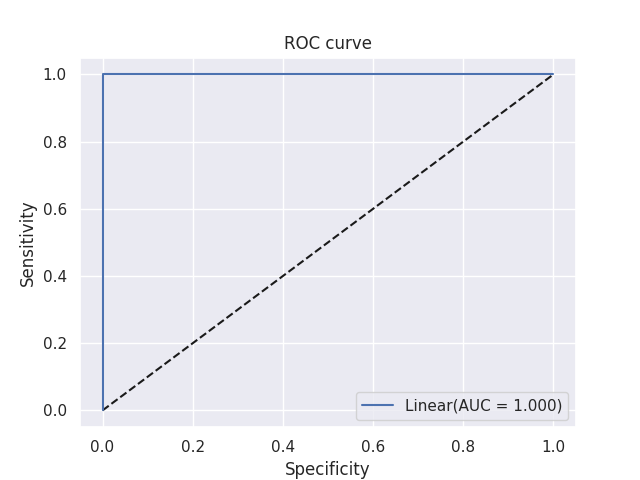
\includegraphics[width=\linewidth]{roc_iris}
      
        \caption{ ROC curve for the test partition of the iris dataset }        
                   
        \label{fig:roc}
    \end{figure}


\textit{In practice, we compute the ROC curve on the test set, rather than on the training
set. Why? Generate the ROC curve for the iris.mat dataset (use tuned gam and sig2 values).Interpret the result}

The receiver operating characteristic (ROC) curves can be used to express the relationship between the sensitivity and the specificity of a classifier along different thresholds. The sensitivity (or true positive rate), plotted on the y-axis, can be described as:

\begin{equation}
TPR = \frac{TP}{TP+FN}
\end{equation}
where TP and FN (true positive and false negative) refer to the number of correctly and incorrectly classified positive instances. Therefore, sensitivity describes the fraction of correctly classified instances over the total number of positive examples. On the other hand, specificity (or false positive rate) is computed as:

\begin{equation}
FPR = \frac{TN}{TN+FP}
\end{equation}
where TN and FP (true negatives) stand for the number correctly and incorrectly classified negative instances. Specificity refers to how accurate the classifier identifies negative cases. By iteratively setting the threshold of the classifier, the curve is produced. Naturally, The area under the curve (AUC) of an ROC plot describes the quality of the classification model. If the AUC score is 1, this means that the model is able to perfectly separate the data. On the other hand, if the area equals 0.5 the classifier has no discriminative power, it simply behaves as a random classifier. The ROC curve is simply computed over the test (or validation set) and not the training set since we are interested in examining the generalization ability of the classifier. As discussed in section 1.3.2, the performance on the test set is used to provide an unbiased evaluation of the final model. 

After tuning the hyperparameters $c$ and $\sigma$, the ROC curve is plotted and shown in Figure ~\ref{ref:roc}. The result shows that is the hyperparameters are properly selected, the obtained classifier can perfectly separate the data, having an AUC score of 1, a FPR of 0 and a TPR of 1. All of the hyperparameters described in Table~\ref{fig:tune1} produce the same result.





\subsubsection{Bayesian framework }
\textit{How do you interpret the colors of the plot? Hint: activate the colorbar of the figure. Change the values of gam and sig2. Visualize and discuss the influence of the parameters on the figure.}



\subsection{Homework Problems}
\subsubsection{Classification of the Ripley dataset}

\begin{figure*}[]
        \begin{subfigure}{0.45\linewidth}
            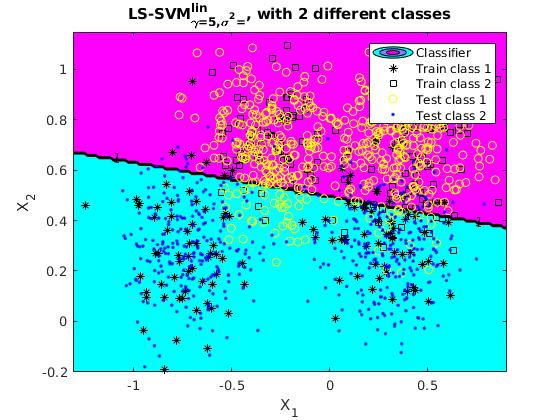
\includegraphics[width=\linewidth]{ripley_linear}
            \caption{Linear kernel}
        \end{subfigure}
        \begin{subfigure}{0.45\linewidth}
            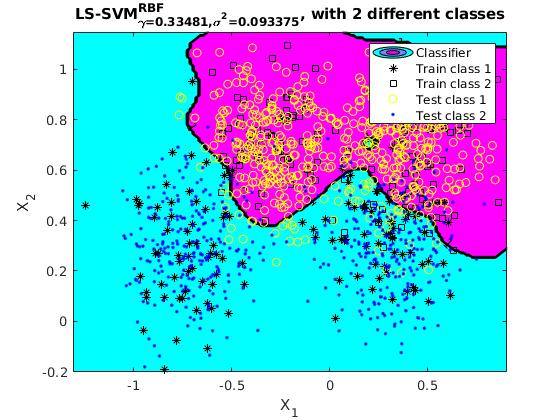
\includegraphics[width=\linewidth]{ripley_rbf}
            \caption{RBF kernel}
        \end{subfigure}
        \centering
	   \begin{subfigure}{0.45\linewidth}
            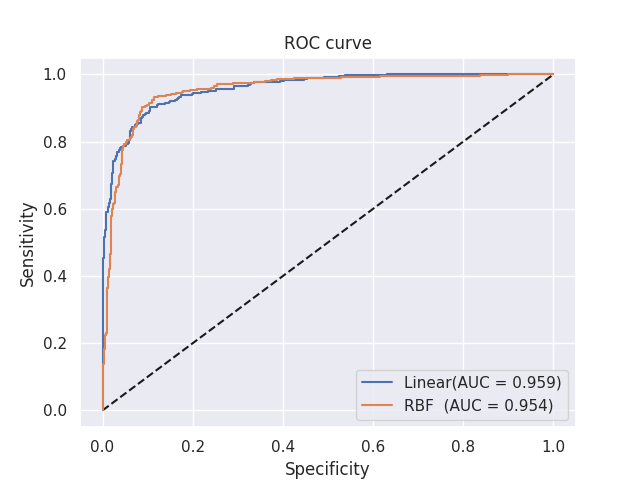
\includegraphics[width=\linewidth]{roc_ripley}
            \caption{Linear kernel}
        \end{subfigure}
         \begin{subfigure}{0.45\linewidth}
            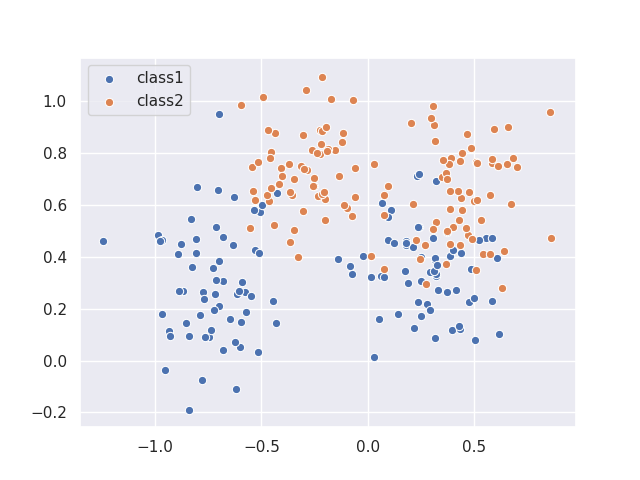
\includegraphics[width=\linewidth]{ripley}
            \caption{The Ripley dataset}
        \end{subfigure}
                   
\caption{Classifying the Ripley dataset}        
        
             
        \label{fig:ripley}
    \end{figure*}
The Ripley dataset consists of a set of input data $x_k \in \mathcal{R}^2 $ and output data $y_k \in \mathcal{R} $ with class labels $y_k \in \{-1,+1 \}$, with 250 data points intended for training and 1000 points intended for test. As illustrated in Figure~\ref{fig:ripley} (d), the two classes seem well separated from each other, although not entirely linearly separable. In the same Figure the results of applying the linear (a) and the RBF (b) kernel are also shown. The linear kernel achieves a classification accuracy of 0.89, while the RBF kernel produces a non-linear decision boundary and reaches an accuracy score of 0.90. For the RBF kernel, the hyperparamteres $c$ and $\gamma$ were tuned using the Nelder-Mead method, as described in section 1.1.6. By plotting the ROC curves in Figure~\ref{fig:ripley} (c), it is is clear that the performance of both kernels is very similar: an AUC score of 0.959 is achieved in the linear case and 0.954 in the RBF case. The conclusion is that any of the two kernels can achieve a good classification performance but since we always opt for the simplest solution the linear kernel is preferred. 


\subsubsection{Classification of the The Breast Cancer dataset}

The Breast cancer dataset consists of 569 examples, with 400 intended for training and 100 for testing. The data points are composed of 30 features that describe metrics suitable for classifying cancer types as benign or malignant. The Bengin class accounts for 62.74\% of the diagnosis class while the malignant class accounts for 37.26\%. The test set follows the same class distribution as 107 out of 169 instances belong to the negative class and 69 to the positive. In Figure~\ref{fig:br} the distributions of the values of the features are shown. Each plot corresponds to one feature. It is observed that the overlap between the two classes is smaller for some of the features (e.g. concave points worst, area worst, concave mean). Moreover, in some cases the values for class -1 are significantly larger (e.g. area se, perimeter se, readius mean, etc). Last but not least, it is shown that in some cases the variance of feature values are remarkable different (e.g. radius worst).

It will be interesting to explore whether we can reduce the dimensionality of the input data points by performing Principal component analysis (PCA). PCA is a dimensionality reduction technique that can be used to project the data observations into a lower dimensional space while maximizing the variance of the projected data. In short,after standardizing the input vectors, the Covariance matrix $C=\{xx^T\}$ that contains all the possible covariance pairs of the initial variables is computed. This is because the covariance matrix expresses how the variables of the observations are varying from the mean with respect to each other. The eigenvectors of this matrix show the directions where the variance is maximal and are called principal components. The amount of variance each principal component carries is expressed by the eigenvalues which can be used to rank the eigenvectors in order of significance. 

While PCA seems a promising solution to reduce the dimensionality while keeping the relevant information, it should be noted that it does not guarantee to always produce a better classification result. This is because the direction of maximal variance does not necessarily make the input data more separable. However, in a lot of cases applying PCA before training can improve the performance or simply allow to reduce the dimension of the input vector. Finally, reducing the dimension of the input vectors can be particularly useful when solving the SVM problem in its primal form where the complexity depends on the dimensionality of the data.

After scaling the data by subtracting the mean observation and by dividing with the standard deviation, a LS-SVM classifier with a linear kernel is trained by using all of the 30 features. The input data is also projected to a different number of principal components and the results and each time  are compared. Table~\ref{fig:brtable} summarizes the results. In the case where all of the 30 features are used, the classifier achieves an accuracy score of 0.9527. It is also shown that by using the first 8 principal components, the classification accuracy is improved from 0.9527 to 0.9645. Interestingly enough, by using only 5 features instead of 30 the result remains the same. The same experiment is repeated for the RBF kernel. First, $\gamma$ and $\sigma^2$ are tuned using the Nelder-Mead method and then the LS-SVM model is trained by using input vectors projected into a different number of principal components. For $\gamma=41.365$ and $\sigma^2=44.38$ and by prjojecting the input evctors to 8 principal components, the best classification score of 0.9882 is achieved. Finally, plotting the ROC curves for both kernels shows that the RBF kernel reaches a very good AUC score of 0.996, while the same score for the linear kernel is at 0.952. To conclude, in this case by performing PCA the relevant information about the features seems to be contained in the projected data and the classification accuracy is improved both in the linear and the RBF case.

\begin{table}\centering
\ra{1.3}
\begin{tabular}{@{}rrrrrrrrrrccrrrcrrr@{}}\toprule
& \multicolumn{4}{c}{Linear} & \phantom{abc}& \multicolumn{2}{c}{RBF} &
\phantom{abc} \\
%\cmidrule{2-10} \cmidrule{12-15} \cmidrule{15-20}
%PC & $2$ & $5$ &$8$ &$10$   &$15$&$30$&  cost\% &&  $\gamma$ & $\sigma^2$ &    cost\% \\ \midrule

 \textbf{2}&   &     0.9172&   &&  &0.9290 &  \\
  \textbf{5}&   &  0.9527 &   &&  &     0.9645 &  \\
   \textbf{8}&   &  \textbf{0.9645} &   &&  &   \textbf{ 0.9882} &  \\
    \textbf{10}&   & 0.9586 &   &&  &  0.9467&  \\
    \textbf{15}&   &  0.9586 &   &&  &   0.9586 &  \\
    \textbf{30}&   &  0.9527 &   &&  &  0.9467 &  \\


\bottomrule
\end{tabular}
\caption{Classification accuracy on the Breast cancer dataset after projecting the input data to 2-30 principal components}
       \label{fig:brtable}
\end{table} 
 
 
\begin{figure*}[]

            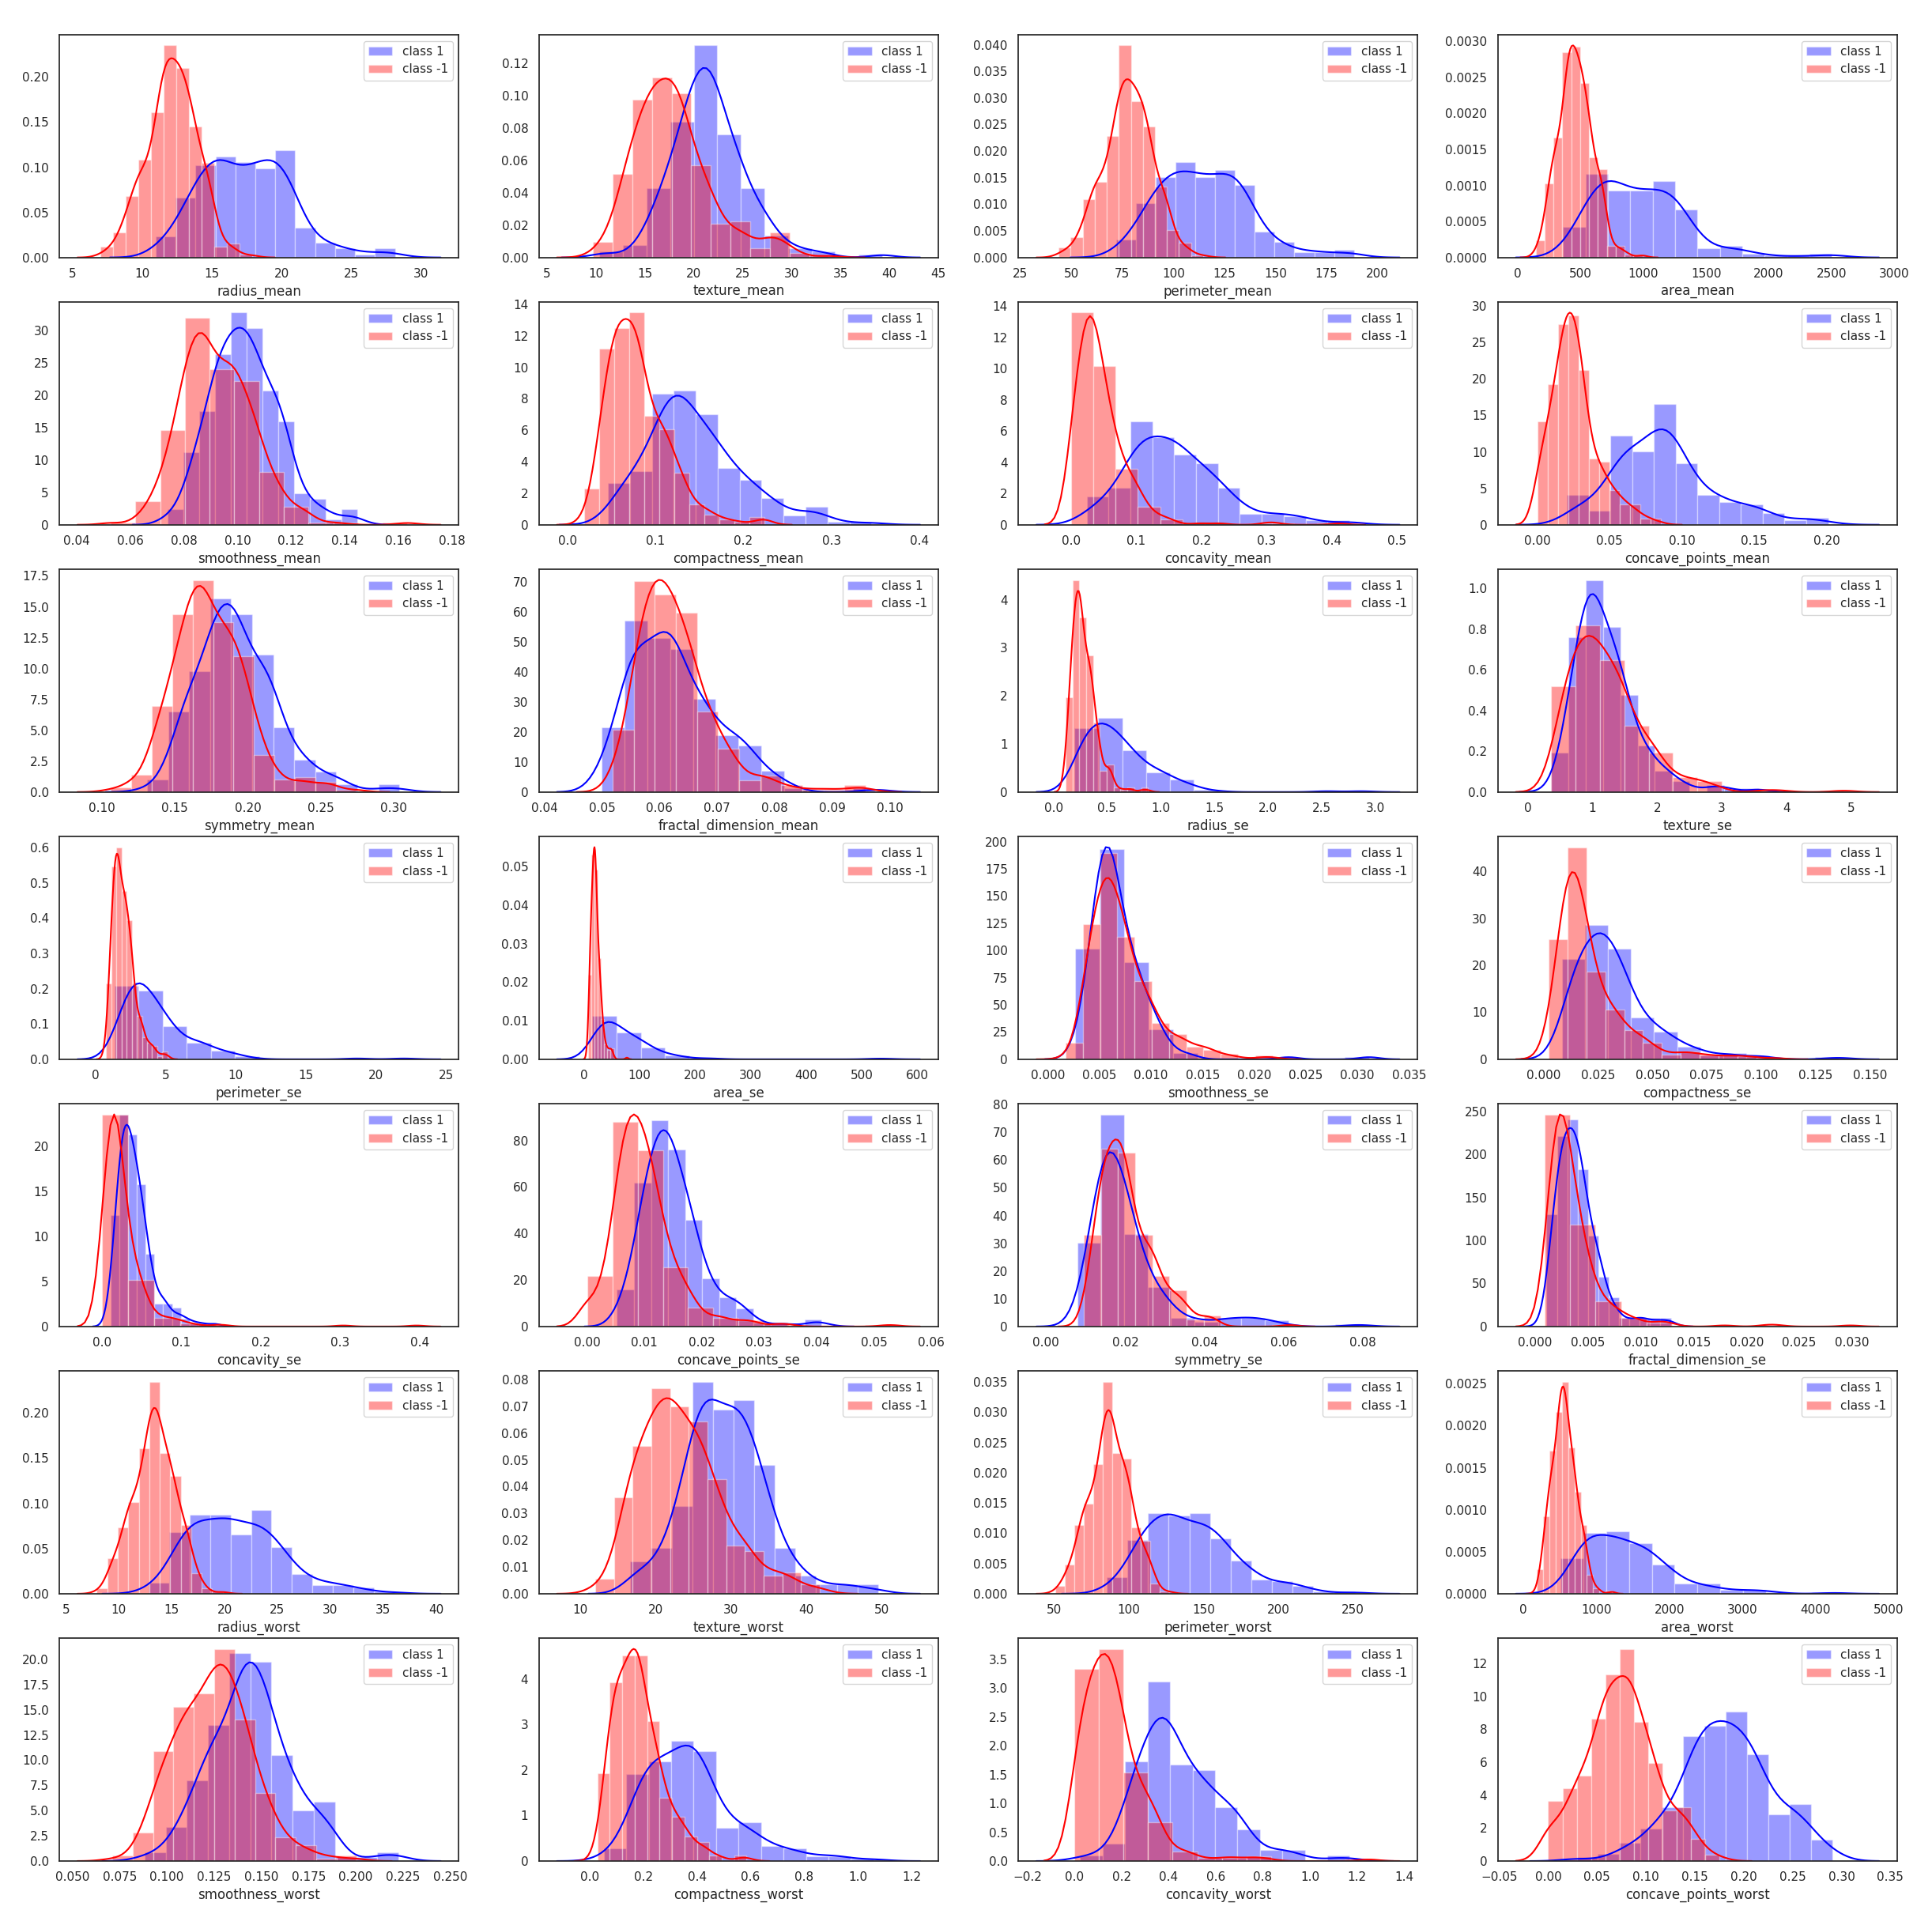
\includegraphics[width=18cm]{features_all}
      
        \caption{Distribution of features for the Breast cancer dataset }        
                   
        \label{fig:br}
    \end{figure*}
\begin{figure*}[]
        \begin{subfigure}{0.45\linewidth}
            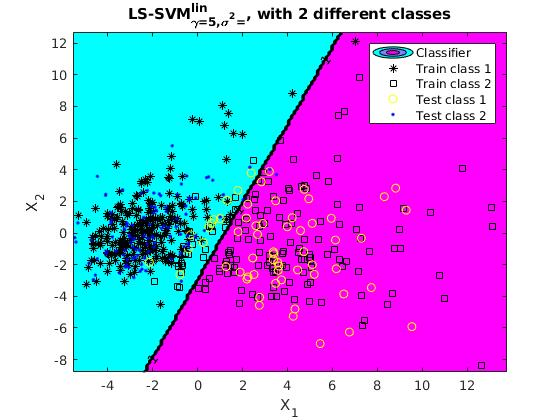
\includegraphics[width=\linewidth]{breast_linear}
            \caption{Linear kernel}
        \end{subfigure}
        \begin{subfigure}{0.45\linewidth}
            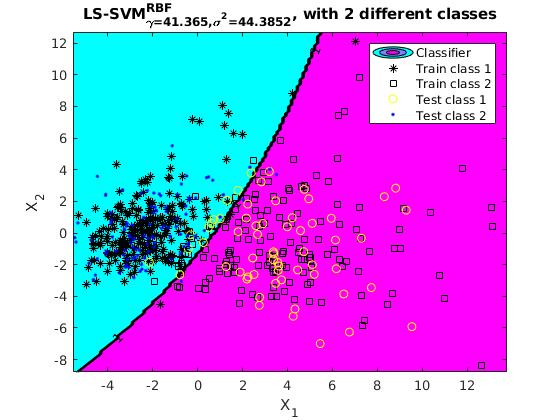
\includegraphics[width=\linewidth]{breast_rbf}
            \caption{RBF kernel}
        \end{subfigure}
        \centering
	   \begin{subfigure}{0.45\linewidth}
            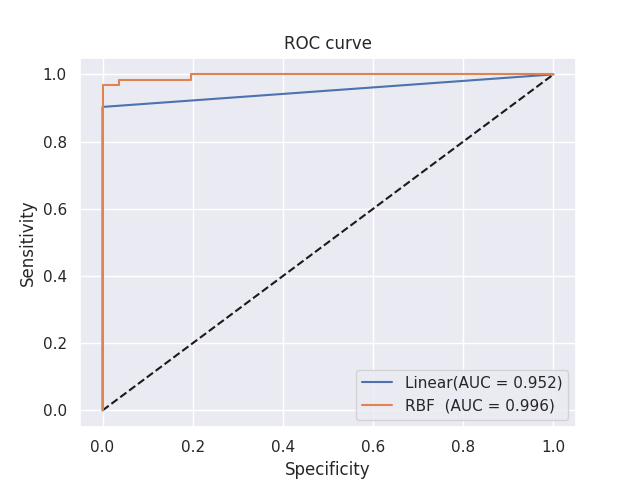
\includegraphics[width=\linewidth]{roc_breast}
            \caption{Linear kernel}
        \end{subfigure}
     
                   
\caption{Classifying the Breast cancer dataset}        
        
             
        \label{fig:brf}
    \end{figure*}



\clearpage



\subsection{Classification of the Diabetes dataset}


The diabetes dataset consists of 468 instances, with 300 intended for training and 168 for testing. The data points are composed of 8 features: Plasma glucose concentration, Diastolic blood pressure, Triceps skin fold thickness, 2-Hour serum insulin, Body mass index, Diabetes pedigree function, Age and finally the number of times the patient was pregnant. Figure~\ref{fig:featuresdiab} shows the distribution of the two classes over the 8 different features. The first thing to note is that there seems to be a high overlap between the distributions of the two classes. Secondly, the feature values of the test partition seem to follow the same distribution as the values in the train partition.

In this exercise, the same methodology as before is followed: First the data points are scaled by subtracting the mean observation and dividing with the standard deviation. Then, a LS-SVM classifier is trained by using all of the 8 features. Next, the input vectors are also projected to 2-8 principal components and results are reported in terms of classification accuracy and ROC curves. Table~\ref{fig:diabable} summarizes the outcome of this experiment. It is shown that in this case PCA does not produce a better classification result, since the best accuracy score is obtained by training with all of the 8 features. For the RBF kernel the classification accuracy is 0.8036 while for the linear case the accuracy result is 0.7440. Figure~\ref{fig:rocdiab} shows the ROC curves for the linear and the RBF kernel. The linear kernel reaches an AUC score of 0.670, while the RBF kernel performs better having an AUC score of 0.844. To conclude, the result is not as satisfying as with the previous two datasets but this is mainly attributed to the fact that there is a high overlap between the values of the available features. 



%\begin{table}\centering
%\ra{1.3}
%\begin{tabular}{@{}rrrrrrrrrrccrrrcrrr@{}}\toprule
%& \multicolumn{4}{c}{Linear} & \phantom{abc}& \multicolumn{2}{c}{RBF} &
%\phantom{abc} \\
%%\cmidrule{2-10} \cmidrule{12-15} \cmidrule{15-20}
%%PC & $2$ & $5$ &$8$ &$10$   &$15$&$30$&  cost\% &&  $\gamma$ & $\sigma^2$ &    cost\% \\ \midrule
%
% \textbf{2}&   &    0.6310&   &&  & 0.6905 &  \\
%  \textbf{3}&   &      0.6429&   &&  &  0.6845 &  \\
%   \textbf{4}&   &      0.6488&   &&  & 0.6786 &  \\
%   \textbf{5}&   &     0.6845&   &&  &    0.7560 &  \\
%  \textbf{6}&   &  0.7143 &   &&  &        0.8036 &  \\
%    \textbf{7}&   &     0.7321 &   &&  &       0.8095 &  \\
%   \textbf{8}&   &  \textbf{ 0.7440} &   &&  &   \textbf{   0.8036} &  \\
%
%
%
%\bottomrule
%\end{tabular}
%\caption{Classification accuracy on the Diabetes dataset after projecting the input data to 2-8 principal components}
%       \label{fig:diabable}
%\end{table} 
%
%\begin{figure}[]
%				\centering
%            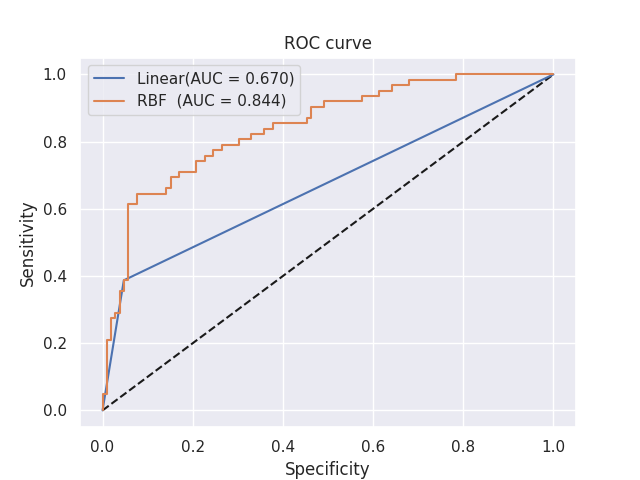
\includegraphics[width=6cm]{roc_diab}
%      
%        \caption{ ROC curve for the test partition of the diabetes dataset }        
%                   
%        \label{fig:rocdiab}
%    \end{figure}
%
%
%
\begin{figure*}[]
\
        \begin{subfigure}{1\linewidth}
            \includegraphics[width=5cm]{diab_train}
            \caption{train set}
        \end{subfigure}
        \begin{subfigure}{1\linewidth}
            \includegraphics[width=5cm]{diab_test}
            \caption{test set}
        \end{subfigure}
        \centering
	
     
             
\caption{Distribution of features for the diabetes dataset}        
        
             
        \label{fig:featuresdiab}
    \end{figure*}


\clearpage
\section{Exercise Session 2}

\end{document}